\chapter{Codigos}\label{anexoA}
\thispagestyle{fancy}
\pagenumbering{arabic}\renewcommand{\thepage}{A.\arabic{page}}
    \section{}
        \subsection{}
        
        
        
\chapter{Desarrollo de formulas teóricas}\label{anexoB}
\thispagestyle{fancy}
\pagenumbering{arabic}\renewcommand{\thepage}{B.\arabic{page}}
    En este anexo se presentan el desarrollo detallado de las fórmulas presentadas en el capitulo \ref{CAP4} 
    
    
\section{Método A}
    \subsection{Modelación cinemática de posición}
        \subsubsection{Cinemática directa}
        
        La cinemática directa busca encontrar la posición del centroide del efector en el espacio cartesiano por medio de la configuración del espacio articular de los actuadores del robot delta.
        \begin{equation*}
             \left(  \theta _{1}, \theta _{2}, \theta _{3} \right)   \rightarrow E_{0} \left( x_{0},y_{0},z_{0} \right)            
        \end{equation*}

        \begin{figure}[htb]
            \centering
            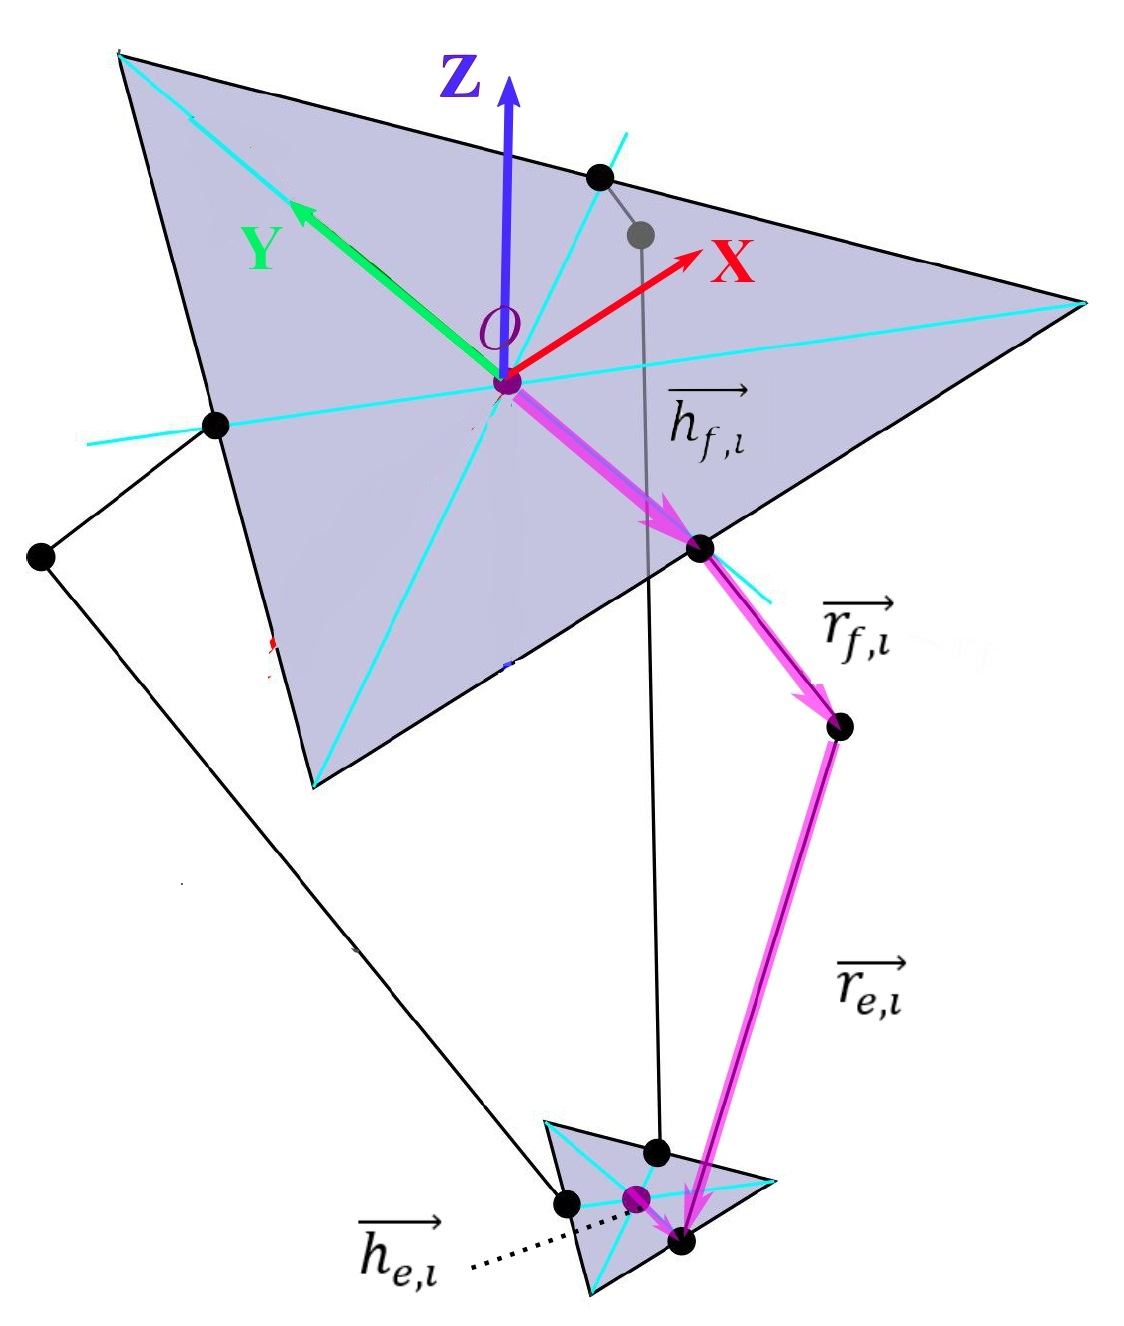
\includegraphics[width=0.45\linewidth]{Main/Chapter4/Images4/DIBUJO10.jpg}
            \caption{Caption}
            \label{fig:ANEXO_MA_C_POS_1}
        \end{figure}

\newpage


        % Multiples imagenes        
            \begin{figure}
             \centering
                  \subfloat[Gatito]{
                   \label{f:gato}
                    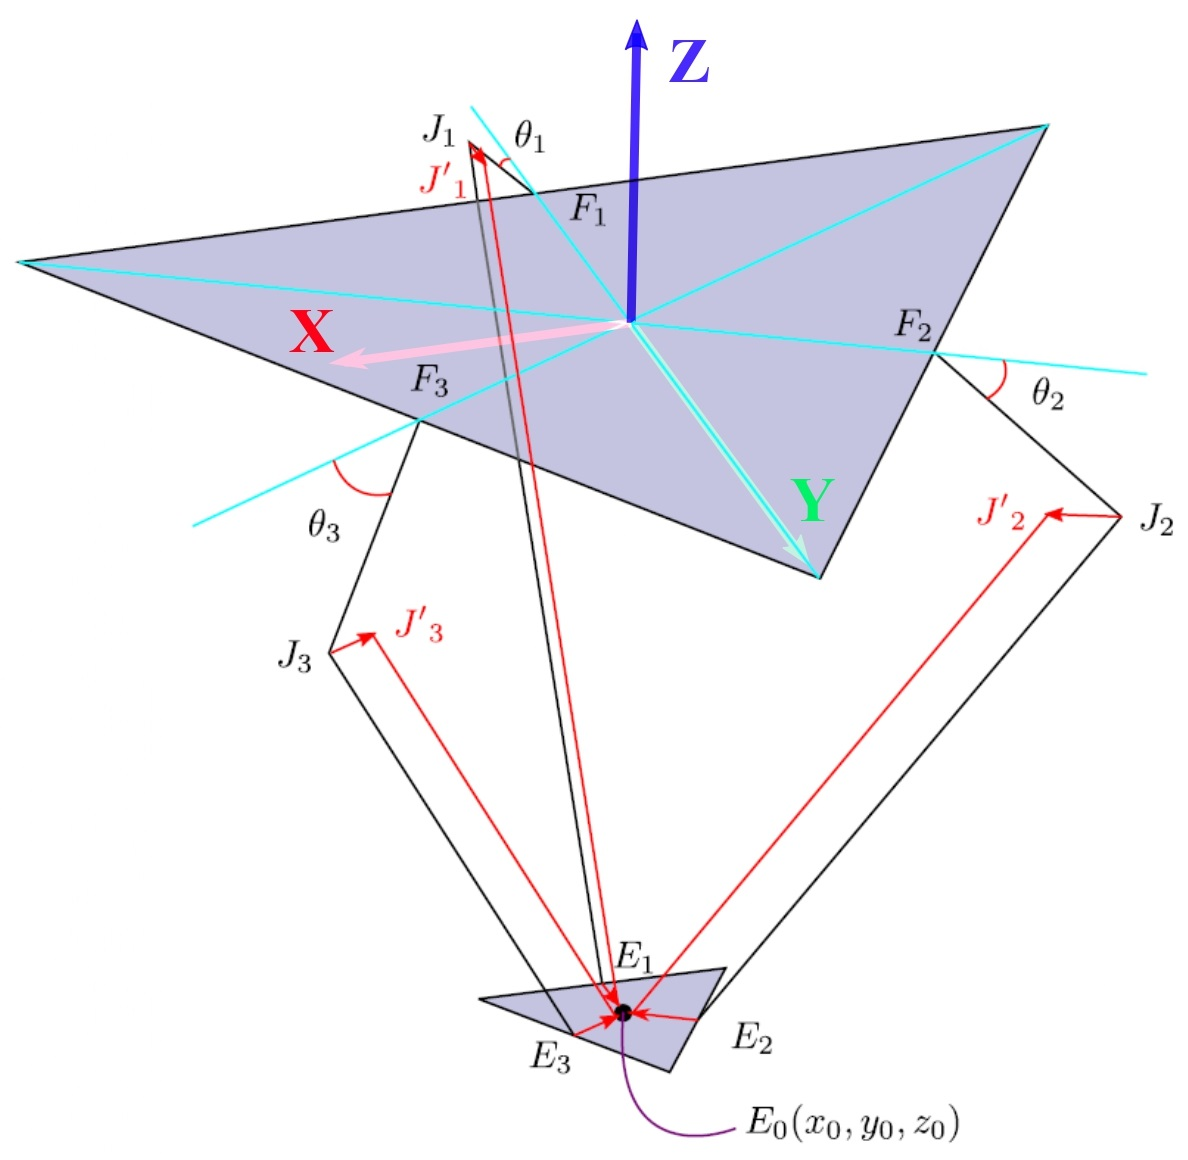
\includegraphics[width=0.5\textwidth]{Main/Chapter4/Images4/DIBUJO7.jpg}}
                  \subfloat[Tigre]{
                   \label{f:tigre}
                    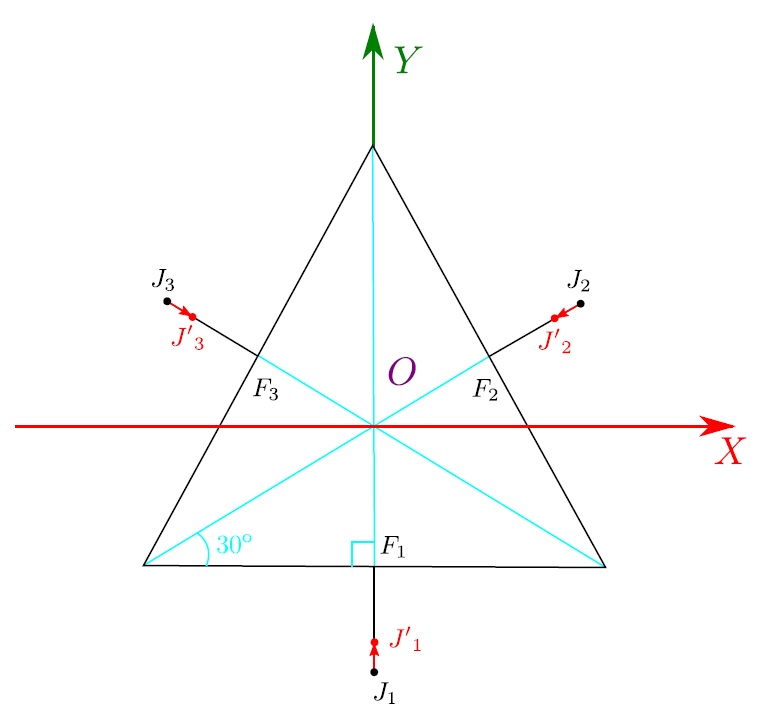
\includegraphics[width=0.5\textwidth]{Main/Chapter4/Images4/DIBUJO8.PNG}}
                 \caption{Múltiples imágenes}
                 \label{f:Desplazamiento_J}
            \end{figure}
            
        Las posiciones en el espacio de los vectores $\overrightarrow{r_{f,i}}$  , que representa los brazos del robot delta, ya están definidos en magnitud y sentido debido a que se conoce los ángulos de los actuadores    $\left(  \theta _{1}, \theta _{2}, \theta _{3} \right)$   y la longitud de los brazos.
        
        Sobre el vector  $\overrightarrow{r_{e,i}}$  ,que representa los antebrazos, solo se conoce el punto inicial  $J_{i}$  que coincide con el extremo del vector   $\overrightarrow{r_{f,i}}$  . En consecuencia, la orientación para cada vector $\overrightarrow{r_{e,i}}$  , está restringido por una esfera con centro en la junta esférica  $J_{i}$ , que conecta el brazo con el antebrazo, con radio equivalente al largo del antebrazo  $r_{e}$ .
        
        Finalmente, para obtener las coordenadas del centroide del efector final   $E_{0} \left( x_{0},y_{0},z_{0} \right)$   , se realiza una traslación de las esferas mencionadas anteriormente. Esta traslación depende de la dirección y longitud del vector   $\overrightarrow{h_{e,i}}$   para cada cadena x respectivamente. Se genera 3 nuevas esferas, con centros en   $J'_{i}$   y de radio equivalente al largo del antebrazo   $r_{e}$  . Estas esferas trasladadas se intersectan en un punto en común, el centroide del efector   $E_{0} \left( x_{0},y_{0},z_{0} \right)$  . Por lo tanto, se calculan las coordenadas del punto  $E_{0} \left( x_{0},y_{0},z_{0} \right)$    realizando un sistema de ecuaciones no lineal con 3 restricciones impuestas por las 3 esferas.
        
        El primer paso para calcular el centroide del efector final  $E_{0}$  es encontrar una manera de representar las posiciones de las juntas  $J_{i}$  (brazo-antebrazo) con los parámetros conocidos. Por medio de geometría básica se pueden determinar otros parámetros para representar el punto   $J_{i}$, como se puede visualizar en la figura \ref{f:Desplazamiento_J}.
        
        El efector tiene forma geométrica de un triángulo equilátero y se tienen las dimensiones de los lados (e), por ende, se puede determinar la magnitud del desplazamiento de las esferas $J_{i}J'_{i}$ de la siguiente manera:
        
        \begin{equation*}
            J_{1}J'_{1}=J_{2}J'_{2}=J_{3}J'_{3}=\frac{e}{2}tan30=\frac{e}{2\sqrt{3}}
        \end{equation*}
    
\newpage
    
            \begin{figure}[htb]
            \centering
            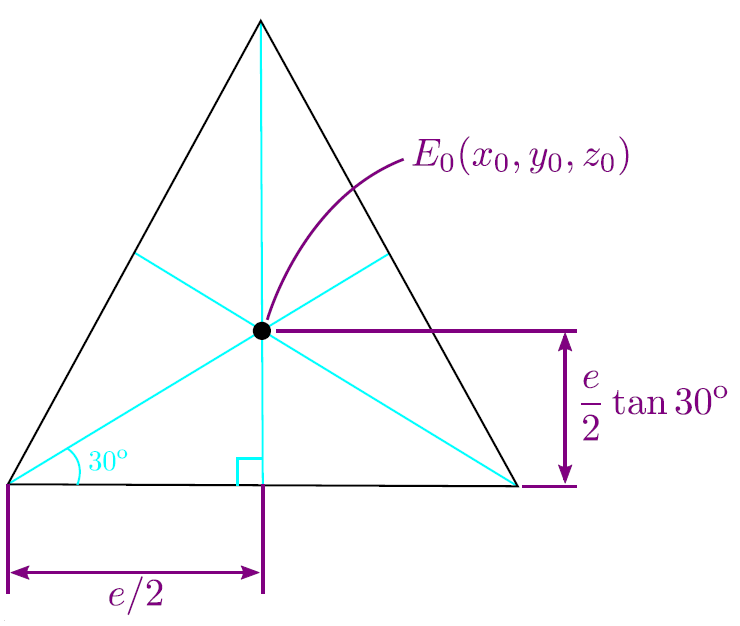
\includegraphics[width=0.5\linewidth]{Main/Chapter4/Images4/DIBUJO9.PNG}
            \caption{Caption}
            \label{fig:ANEXO_MA_C_POS_2}
        \end{figure}

        Similar a como se calcula el desplazamiento de las esferas $J_{i}~J'_{i}$, se determina la magnitud de la distancia entre el centroide de la base fija y la posición de los actuadores $OF_{i}$ :
        
        \begin{equation*}
            OF_{1}=OF_{2}=OF_{3}=\frac{f}{2}tan30=\frac{f}{2\sqrt{3}}
        \end{equation*}
        
        La distancia perpendicular entre el plano que contiene la base fija y el punto donde se encuentra las juntas esféricas $J_{i}$  que unen los brazos con sus antebrazos, está en función de cada ángulo de los actuadores $i=1,2,3$, dada por la siguiente ecuación:
        
        \begin{equation*}
            F_iJ_i=r_fcos(\theta_i) , \forall i=1,2,3
        \end{equation*}
        
        Por lo tanto, los centros de las esferas de radio $r_e$ que se intersectan en el centroide  $E_{0} \left( x_{0},y_{0},z_{0} \right)$ del efector son:
        
                \begin{center}
        \renewcommand{\arraystretch}{2.5}
        
            \begin{table}[H]
            \centering
            \begin{tabular}{c c } 
                 \hline
                 \textbf {Centros esferas}\\ [0.1ex] 
                 \hline\hline
                         $\left(x_1,y_1,z_1\right)$ =
                         ${J^'}_1\left(0,\left[-\frac{f-e}{2\sqrt{3}}-r_f{\mathrm{cos} \left({\theta }_1\right)\ }\right],-r_f{\mathrm{sin} \left({\theta }_1\right)\ }\right)$\\ 
                \hline
                          $\left(x_2,y_2,z_2\right)$ = ${J^'}_2\left(\left[\frac{f-e}{2\sqrt{3}}+r_f{\mathrm{cos} \left({\theta }_2\right)\ }\right]\mathrm{cos}\mathrm{}(30{}^\circ ),\left[\frac{f-e}{2\sqrt{3}}+r_f{\mathrm{cos} \left({\theta }_2\right)\ }\right]\mathrm{sin}\mathrm{}(30{}^\circ ),-r_f{\mathrm{sin} \left({\theta }_2\right)\ }\right)$  \\
                \hline
                           $\left(x_3,y_3,z_3\right)$ = ${J^'}_3\left(-\left[\frac{f-e}{2\sqrt{3}}+r_f{\mathrm{cos} \left({\theta }_3\right)\ }\right]\mathrm{cos}\mathrm{}(30{}^\circ ),\left[\frac{f-e}{2\sqrt{3}}+r_f{\mathrm{cos} \left({\theta }_3\right)\ }\right]\mathrm{sin}\mathrm{}(30{}^\circ ),-r_f{\mathrm{sin} \left({\theta }_3\right)\ }\right)$ \\ [1ex] 
                 \hline
            \end{tabular}
            \caption{Referencias del dibujo}
            \label{tab:anexo_tabla_3}
            \end{table}
        \end{center}
        
        \newpage

        
        A consecuencia de las extensas representaciones de los centros parametrizados, se resumen las ecuaciones cartesianas de las esferas de la siguiente forma:
        
        \begin{equation*}
              \left\{ \begin{array}{c}
            	 \left( x-x_{1} \right) ^{2}+ \left( y-y_{1} \right) ^{2} + \left( z-z_{1} \right) ^{2}= r_{e}^{2}~\\
            	 \left( x-x_{2} \right) ^{2}+ \left( y-y_{2} \right) ^{2} + \left( z-z_{2} \right) ^{2}= r_{e}^{2}\\
            	 \left( x-x_{3} \right) ^{2}+ \left( y-y_{3} \right) ^{2} +x \left( z-z_{3} \right) ^{2}= r_{e}^{2}\\
            \end{array} \right.   
        \end{equation*}

        Los centros  $\left( x_{1},y_{1},z_{1} \right) ,~ \left( x_{2},y_{2},z_{2} \right) ,~ \left( x_{3},y_{3},z_{3} \right)$  se muestran en la tabla \ref{tab:anexo_tabla_3}.
        

        Ampliando las ecuaciones anteriores:
        
        \begin{equation*}
              \left\{ \begin{array}{c}
        	x^{2}+y^{2} +z^{2}-2x_{1}x-2y_{1}y-2z_{1}z = r_{e}^{2}- x_{1}^{2}- y_{1}^{2}-z_{1}^{2}\\
        	x^{2}+y^{2} +z^{2}-2x_{2}x-2y_{2}y-2z_{2}z = r_{e}^{2}- x_{2}^{2}- y_{2}^{2}-z_{2}^{2}\\
        	x^{2}+y^{2} +z^{2}-2x_{3}x-2y_{3}y-2z_{3}z = r_{e}^{2}- x_{3}^{2}- y_{3}^{2}-z_{3}^{2}\\
            \end{array} \right.   
        \end{equation*}
        
        Se crean nuevas constantes  $w_{i}~ i  \in  \{ 1,2,3 \}$  con el objetivo de simplificar las ecuaciones anteriores:
        
        \begin{equation*}
         w_{i}= x_{i}^{2}+y_{i}^{2} +z_{i}^{2}
        \end{equation*}

        Reemplazando $w_{i}$ en las ecuaciones:
        
        \begin{equation*}
            \left\{ \begin{array}{c}
            	x^{2}+y^{2} +z^{2}-2x_{1}x-2y_{1}y-2z_{1}z = r_{e}^{2}- w_{1}~~  \left( 1 \right) \\
            	x^{2}+y^{2} +z^{2}-2x_{2}x-2y_{2}y-2z_{2}z = r_{e}^{2}- w_{2}~~  \left( 2 \right) \\
            	x^{2}+y^{2} +z^{2}-2x_{3}x-2y_{3}y-2z_{3}z = r_{e}^{2}- w_{3}~~  \left( 3 \right) \\
                \end{array} \right.   
        \end{equation*}
        
        Restando las ecuaciones $(1)$-$(2)$, $(1)$-$(3)$ y $(2)$-$(3)$
        
        \begin{equation*}
            \left\{ \begin{array}{c}
        	 \left( x_{1}-x_{2} \right) x+ \left( y_{1}-y_{2} \right) y+ \left( z_{1}-z_{2} \right) z= \frac{ \left( w_{1} - w_{2} \right) }{2}~~  \left( 4 \right) \\
        	 \left( x_{1}-x_{3} \right) x+ \left( y_{1}-y_{3} \right) y+ \left( z_{1}-z_{3} \right) z= \frac{ \left( w_{1} - w_{3} \right) }{2}~~  \left( 5 \right) \\
        	 \left( x_{2}-x_{3} \right) x+ \left( y_{2}-y_{3} \right) y+ \left( z_{2}-z_{3} \right) z= \frac{ \left( w_{2} - w_{3} \right) }{2}~~  \left( 6 \right) \\
                \end{array} \right.   
        \end{equation*}
        
        Los sistemas de ecuaciones no lineales son complejos, por lo que se proponen los siguientes pasos para encontrar la solución $(x, y, z)$.
        
        \begin{enumerate}
        	\item {Se despeja $x$ de una de las ecuaciones (4), (5) o (6) en función de $z$, es decir,$x(z)$.}
        	\item {Se despeja $y$ de una de las ecuaciones (4), (5) o (6) (no elegida anteriormente) en función de $z$, es decir,$y(z)$.}
        	\item {Con las 2 ecuaciones encontradas en los pasos 1 y 2 en función de $z$, se reemplazan en (1) para encontrar la solución de $z$, en consecuencia se puede obtiene finalmente la solución $(x, y, z)$.}
        \end{enumerate}
        
        \newpage


        Paso 1:
        
        Multiplicado $(5)\ast \frac{( y_{2}-y_{1}) }{(y_{1}-y_{3})}$: 

        \begin{equation*}
                \frac{ \left( y_{2}-y_{1} \right) }{ \left( y_{1}-y_{3} \right) } \left( x_{1}-x_{3} \right) x+ \left( y_{2}-y_{1} \right) y+\frac{ \left( y_{2}-y_{1} \right) }{ \left( y_{1}-y_{3} \right) } \left( z_{1}-z_{3} \right) z= \frac{ \left( y_{2}-y_{1} \right) }{ \left( y_{1}-y_{3} \right) }\frac{ \left( w_{1} - w_{3} \right) }{2} ~~\left( 7 \right)
        \end{equation*}
        
        Sumando $(4) +(7)$ para eliminar $y$:
        \begin{multline*}
             \left[ \frac{ \left( y_{2}-y_{1} \right) }{ \left( y_{1}-y_{3} \right) } \left( x_{1}-x_{3} \right) +  \left( x_{1}-x_{2} \right)  \right] x+ \left[ \frac{ \left( y_{2}-y_{1} \right) }{ \left( y_{1}-y_{3} \right) } \left( z_{1}-z_{3} \right) + \left( z_{1}-z_{2} \right)  \right] z= \\ \frac{ \left( y_{2}-y_{1} \right) }{ \left( y_{1}-y_{3} \right) }\frac{ \left( w_{1} - w_{3} \right) }{2}+\frac{ \left( w_{1} - w_{2} \right) }{2}~~~ \left( 8 \right)            
        \end{multline*}

        Despejando $x$ en función de $z$ en la ecuación $(8)$ para dar como resultado  $x= a_{1}z+ b_{1}$:

        \begin{multline*}
             \left[ \frac{ \left( y_{2}-y_{1} \right) }{ \left( y_{1}-y_{3} \right) } \left( x_{1}-x_{3} \right) +  \left( x_{1}-x_{2} \right)  \right] x=\\- \left[ \frac{ \left( y_{2}-y_{1} \right) }{ \left( y_{1}-y_{3} \right) } \left( z_{1}-z_{3} \right) + \left( z_{1}-z_{2} \right)  \right] z+ \frac{ \left( y_{2}-y_{1} \right) }{ \left( y_{1}-y_{3} \right) }\frac{ \left( w_{1} - w_{3} \right) }{2}+\frac{ \left( w_{1} - w_{2} \right) }{2}~~~ \left( 9 \right) 
        \end{multline*}

        Multiplicando (9) $\ast$ $\left( y_{1}-y_{3} \right)$:
        \begin{multline*}
             \left[  \left( y_{2}-y_{1} \right)  \left( x_{1}-x_{3} \right) +  \left( y_{1}-y_{3} \right)  \left( x_{1}-x_{2} \right)  \right] x=\\- \left[  \left( y_{2}-y_{1} \right)  \left( z_{1}-z_{3} \right) + \left( y_{1}-y_{3} \right)  \left( z_{1}-z_{2} \right)  \right] z+\\  \left( y_{2}-y_{1} \right) \frac{ \left( w_{1} - w_{3} \right) }{2}+ \left( y_{1}-y_{3} \right) \frac{ \left( w_{1} - w_{2} \right) }{2}~~~ \left( 10 \right) 
        \end{multline*}
        
            Multiplicando (10) $\ast$   $\frac{1}{ \left[  \left( y_{2}-y_{1} \right)  \left( x_{1}-x_{3} \right) +  \left( y_{1}-y_{3} \right)  \left( x_{1}-x_{2} \right)  \right] }$
            
        \begin{multline*}
             x= \left[ \frac{-1}{ \left[  \left( y_{2}-y_{1} \right)  \left( x_{1}-x_{3} \right) +  \left( y_{1}-y_{3} \right)  \left( x_{1}-x_{2} \right)  \right] }\ast \left[  \left( y_{2}-y_{1} \right)  \left( z_{1}-z_{3} \right) + \left( y_{1}-y_{3} \right)  \left( z_{1}-z_{2} \right)  \right]  \right] z\\+ \left[  \left( \frac{1}{ \left[  \left( y_{2}-y_{1} \right)  \left( x_{1}-x_{3} \right) +  \left( y_{1}-y_{3} \right)  \left( x_{1}-x_{2} \right)  \right] } \right)\right. \\  \left.\ast \left( \left(y_{2}-y_{1} \right) \frac{ \left( w_{1} - w_{3} \right) }{2}+ \left( y_{1}-y_{3} \right) \frac{ \left( w_{1} - w_{2} \right) }{2}\right)\right] ~ \left( 11 \right) 
        \end{multline*}
        
        Creando $d$ para simplificar las ecuaciones:
        \begin{align*}
              d&= - \left[  \left( y_{2}-y_{1} \right)  \left( x_{1}-x_{3} \right) +  \left( y_{1}-y_{3} \right)  \left( x_{1}-x_{2} \right)  \right] \\
             \Longrightarrow d&= - \left[  \left( y_{2}x_{1}-y_{1}x_{1}- y_{2}x_{3}+y_{1}x_{3} \right) +  \left( y_{1}x_{1}-y_{3}x_{1}-y_{1}x_{2}+y_{3}x_{2} \right)  \right]\\
             \Longrightarrow d&= - \left[ y_{2}x_{1}-y_{3}x_{1}- y_{2}x_{3}+y_{1}x_{3}+ -y_{1}x_{2}+y_{3}x_{2} \right] \\
             \Longrightarrow d&=- \left[  \left( y_{2}-y_{3} \right) x_{1}+ \left( y_{3}-y_{1} \right) x_{2}+ \left( y_{1}- y_{2} \right) x_{3} \right] \\
             \Longrightarrow d&=- \left[  \left( y_{2}-y_{3} \right) x_{1}+ \left( y_{3}-y_{1} \right) x_{2}+ \left( y_{1}- y_{2} \right) x_{3} \right] \\
             \Longrightarrow d&= \left( y_{2}- y_{1} \right) x_{3}- \left( y_{3}-y_{1} \right) x_{2}-  \left( y_{2}-y_{3} \right) x_{1}~~  \left( 12 \right)             
        \end{align*}
        
        \newpage

        Agrupando términos de la siguiente manera:
        \begin{equation*}
            x= a_{1}z+ b_{1}
        \end{equation*}

         Donde  $a_{1}$:
        
        \begin{align*}
         a_{1}&=\frac{ \left( y_{2}-y_{1} \right)  \left( z_{1}-z_{3} \right) + \left( y_{1}-y_{3} \right)  \left( z_{1}-z_{2} \right) }{d}\\
         \Longrightarrow a_{1}&=\frac{ \left( z_{2}-z_{1} \right)  \left( y_{3}-y_{1} \right) - \left( z_{3}-z_{1} \right)  \left( y_{2}-y_{1} \right) }{d}~  \left( 13 \right) 
        \end{align*}
        
        Donde  $b_{1}$:

        \begin{align*}
             b_{1}&= \left( \frac{1}{ \left[  \left( y_{2}-y_{1} \right)  \left( x_{1}-x_{3} \right) +  \left( y_{1}-y_{3} \right)  \left( x_{1}-x_{2} \right)  \right] } \right) \\ &\ast \left(  \left( y_{2}-y_{1} \right) \frac{ \left( w_{1} - w_{3} \right) }{2}+ \left( y_{1}-y_{3} \right) \frac{ \left( w_{1} - w_{2} \right) }{2}~~ \right)    \\                 
             b_{1}&= \left( \frac{1}{2\ast \left( -d \right) } \right) \ast \left[  \left( w_{2} - w_{1} \right)  \left( y_{3}-y_{1} \right) - \left( w_{3} - w_{1} \right)  \left( y_{2}-y_{1} \right)  \right] ~  \left( 14 \right) 
        \end{align*}

        
Paso 2:
        
        Multiplicado $(5)\ast\frac{ \left( x_{2}-x_{1} \right) }{ \left( x_{1}-x_{3} \right) }$:

        \begin{equation*}
             \left( x_{2}-x_{1} \right) x+\frac{ \left( x_{2}-x_{1} \right) }{ \left( x_{1}-x_{3} \right) } \left( y_{1}-y_{3} \right) y+\frac{ \left( x_{2}-x_{1} \right) }{ \left( x_{1}-x_{3} \right) } \left( z_{1}-z_{3} \right) z= \frac{ \left( x_{2}-x_{1} \right) }{ \left( x_{1}-x_{3} \right) }\frac{ \left( w_{1} - w_{3} \right) }{2}~~ \left( 15 \right) 
        \end{equation*}

        Sumando $(4) +(15)$ para eliminar $y$:
        
        \begin{multline*}
             \left[ \frac{ \left( x_{2}-x_{1} \right) }{ \left( x_{1}-x_{3} \right) } \left( y_{1}-y_{3} \right) +  \left( y_{1}-y_{2} \right)  \right] y+ \left[ \frac{ \left( x_{2}-x_{1} \right) }{ \left( x_{1}-x_{3} \right) } \left( z_{1}-z_{3} \right) + \left( z_{1}-z_{2} \right)  \right] z= \\ \left[ \frac{ \left( x_{2}-x_{1} \right) }{ \left( x_{1}-x_{3} \right) }\frac{ \left( w_{1} - w_{3} \right) }{2}+\frac{ \left( w_{1} - w_{2} \right) }{2} \right] ~~~ \left( 16 \right)
        \end{multline*}

        Despejando $y$ en función de $z$ en la ecuación $(16)$ para dar como resultado $y= a_{2}z+ b_{2}$:

        \begin{multline*}
             \left[ \frac{ \left( x_{2}-x_{1} \right) }{ \left( x_{1}-x_{3} \right) } \left( y_{1}-y_{3} \right) +  \left( y_{1}-y_{2} \right)  \right] y=\\- \left[ \frac{ \left( x_{2}-x_{1} \right) }{ \left( x_{1}-x_{3} \right) } \left( z_{1}-z_{3} \right) + \left( z_{1}-z_{2} \right)  \right] z+  \left[ \frac{ \left( x_{2}-x_{1} \right) }{ \left( x_{1}-x_{3} \right) }\frac{ \left( w_{1} - w_{3} \right) }{2}+\frac{ \left( w_{1} - w_{2} \right) }{2} \right] ~~~ \left( 17 \right)
        \end{multline*}

\newpage


        Multiplicando (17) $\ast$ $\left( x_{1}-x_{3} \right)$
        \begin{multline*}
             \left[  \left( x_{2}-x_{1} \right)  \left( y_{1}-y_{3} \right) +  \left( x_{1}-x_{3} \right)  \left( y_{1}-y_{2} \right)  \right] y=\\- \left[  \left( x_{2}-x_{1} \right)  \left( z_{1}-z_{3} \right) + \left( x_{1}-x_{3} \right)  \left( z_{1}-z_{2} \right)  \right] z+\\ \left[  \left( x_{2}-x_{1} \right) \frac{ \left( w_{1} - w_{3} \right) }{2}+ \left( x_{1}-x_{3} \right) \frac{ \left( w_{1} - w_{2} \right) }{2} \right]  \left( 18 \right)
        \end{multline*}
        
        Multiplicando (18) $\ast$ $\frac{1}{ \left[  \left( x_{2}-x_{1} \right)  \left( y_{1}-y_{3} \right) +  \left( x_{1}-x_{3} \right)  \left( y_{1}-y_{2} \right)  \right] }= $(18)$\ast \frac{1}{d} $

        \begin{multline*}
             y=\frac{- \left[  \left( x_{2}-x_{1} \right)  \left( z_{1}-z_{3} \right) + \left( x_{1}-x_{3} \right)  \left( z_{1}-z_{2} \right)  \right] }{d}z+\\ \left[  \left( x_{2}-x_{1} \right) \frac{ \left( w_{1} - w_{3} \right) }{2d}+ \left( x_{1}-x_{3} \right) \frac{ \left( w_{1} - w_{2} \right) }{2d} \right]  \left( 19 \right)
        \end{multline*}

        Agrupando términos de la siguiente manera:
        \begin{equation*}
            y= a_{2}z+ b_{2}
        \end{equation*}

        Donde $a_{2}$:
        
        \begin{align*}
         a_{2}&=\frac{- \left[  \left( x_{2}-x_{1} \right)  \left( z_{1}-z_{3} \right) + \left( x_{1}-x_{3} \right)  \left( z_{1}-z_{2} \right)  \right] }{d} \\
         \Longrightarrow ~~~ a_{2}&=\frac{-1}{d}\ast \left[  \left( z_{2}-z_{1} \right) x_{3}- \left( z_{3}-z_{1} \right) x_{2}+ \left( z_{3}-z_{2} \right) x_{1} \right]   \left( 19 \right) 
        \end{align*}
        
        Donde $b_{2}$:

        \begin{align*}
             b_{2}&= \left[  \left( x_{2}-x_{1} \right) \frac{ \left( w_{1} - w_{3} \right) }{2d}+ \left( x_{1}-x_{3} \right) \frac{ \left( w_{1} - w_{2} \right) }{2d} \right]\\
             \Longrightarrow ~ b_{2}&=\frac{1}{2d}\ast \left[  \left( x_{1}-x_{3} \right)  \left( w_{1} - w_{2} \right) + \left( x_{2}-x_{1} \right)  \left( w_{1} - w_{3} \right)  \right]\\
             \Longrightarrow ~ b_{2}&=\frac{1}{2d}\ast \left[  \left( x_{1}w_{1}-x_{3}w_{1}-x_{1}w_{2}+x_{3}w_{2} \right) + \left( x_{2}w_{1}-x_{1}w_{1}-x_{2}w_{3}+x_{1}w_{3} \right)  \right]\\
             \Longrightarrow ~ b_{2}&=\frac{1}{2d}\ast \left[  \left( -x_{3}w_{1}+x_{3}w_{2} \right) + \left( x_{2}w_{1}-x_{2}w_{3} \right) + \left( x_{1}w_{3}-x_{1}w_{2} \right) \right]\\
            \Longrightarrow b_{2}&=\frac{1}{2d}\ast \left[  \left( w_{2}-w_{1} \right) x_{3}- \left( w_{3}-w_{1} \right) x_{2}+ \left( w_{3}-w_{2} \right) x_{1}\right] ~  \left( 20 \right)  \\ 
        \end{align*}

\newpage


        Paso 3:

        Sustituyendo $x= a_{1}z+ b_{1}$ y $y= a_{2}z+ b_{2}$ en $(1)$:

        \vspace{-1em}
        \begin{multline*}
             \left( a_{1}z+ b_{1} \right) ^{2}+ \left( a_{2}z+ b_{2} \right) ^{2} +z^{2}-2x_{1} \left( a_{1}z+ b_{1} \right) -2y_{1} \left( a_{2}z+ b_{2} \right) -2z_{1}z =\\ r_{e}^{2}- x_{1}^{2}- y_{1}^{2}-z_{1}^{2}             
        \end{multline*}


        Reordenando $z$ como una función cuadrática:

        \begin{align*}
               \Longrightarrow&\left( a_{1}^{2}z^{2}+2a_{1}b_{1}z+~b_{1}^{2} \right) + \left( a_{2}^{2}z^{2}+2a_{2}b_{2}z+b_{2}^{2} \right)  +z^{2}-\\&2x_{1} \left( a_{1}z+ b_{1} \right) -2y_{1} \left( a_{2}z+ b_{2} \right) -2z_{1}z = r_{e}^{2}- x_{1}^{2}- y_{1}^{2}-z_{1}^{2}\\
              \Longrightarrow& ~  \left( a_{1}^{2}+a_{2}^{2}+1 \right) z^{2}+ \left( 2a_{1}b_{1}+2a_{2}b_{2}-2x_{1}a_{1}-2y_{1}a_{2}-2z_{1} \right) z+\\& \left( ~b_{1}^{2}+b_{2}^{2}-2x_{1}b_{1}-2y_{1}b_{2} \right) = r_{e}^{2}- x_{1}^{2}- y_{1}^{2}-z_{1}^{2} \\
               \Longrightarrow& ~  \left( a_{1}^{2}+a_{2}^{2}+1 \right) z^{2}+ \left( 2a_{1}b_{1}+2a_{2}b_{2}-2x_{1}a_{1}-2y_{1}a_{2}-2z_{1} \right) z+\\& \left( ~b_{1}^{2}+b_{2}^{2}-2x_{1}b_{1}-2y_{1}b_{2}- r_{e}^{2}+ x_{1}^{2}+ y_{1}^{2}+z_{1}^{2} \right) =0 \\         
             \Longrightarrow& ~  \left( a_{1}^{2}+a_{2}^{2}+1 \right) z^{2}+2 \left( a_{1} \left( b_{1}-x_{1} \right) +a_{2} \left( b_{2}-y_{1} \right) -z_{1} \right) z+\\& \left( ~b_{1}^{2}+b_{2}^{2}-2y_{1}b_{2}+ y_{1}^{2}-2x_{1}b_{1}+ x_{1}^{2}+z_{1}^{2}- r_{e}^{2} \right) =0\\
            \Longrightarrow &~  \left( a_{1}^{2}+a_{2}^{2}+1 \right) z^{2}+2 \left( a_{1} \left( b_{1}-x_{1} \right) +a_{2} \left( b_{2}-y_{1} \right) -z_{1} \right) z+\\& \left(  \left( b_{1}-x_{1} \right) ^{2}+ \left( b_{2}-y_{1} \right) ^{2}+z_{1}^{2}- r_{e}^{2} \right) =0
        \end{align*}

        Agregando nuevas constantes para simplificar la expresión anterior:

        \begin{equation*}
         A\ast z^{2}+B\ast z+C=0 
        \end{equation*}

        Donde:
        \begin{align*}
         A=& a_{1}^{2}+a_{2}^{2}+1 \\
         B=& 2 \left[ a_{1} \left( b_{1}-x_{1} \right) +a_{2} \left( b_{2}-y_{1} \right) -z_{1} \right]  \\
        C=&  \left( b_{1}-x_{1} \right) ^{2}+ \left( b_{2}-y_{1} \right) ^{2}+z_{1}^{2}- r_{e}^{2} 
        \end{align*}
        
        Resolviendo la ecuación de segundo grado se obtiene:
        
        \begin{equation*}
         z= \frac{-B  \pm  \sqrt[]{ B^{2} - 4AC }}{2\ast A} 
        \end{equation*}
        
        Se puede apreciar que z tiene dos soluciones, pero solo una es físicamente posible (la raíz de la ecuación que tenga coordenada z mayor valor negativa), $z= \frac{-B-\sqrt[]{  B^{2}  -4AC }}{2\ast A}$. Por lo tanto, la solución del sistema de ecuaciones es:

        \begin{equation*}
                 (x,y,z)=\left( a_{1}z+ b_{1},a_{2}z+ b_{2},z \right) = \left( a_{1}z+ b_{1},a_{2}z+ b_{2},\frac{-B- \sqrt[]{ B^{2}  -  4AC  }}{2\ast A} \right)      
        \end{equation*}
        


\newpage
        
        
        
        
    \subsubsection{Cinemática inversa}
        
        El objetivo de la cinemática inversa es encontrar los ángulos de los actuadores del robot delta conociendo la posición del centroide de su efector final:
        
        \begin{equation*}
        E_{0} \left( x_{0},y_{0},z_{0} \right) ~~  \rightarrow  \left(  \theta _{1}, \theta _{2}, \theta _{3} \right) 
        \end{equation*}

        \begin{figure}[htb]
            \centering
            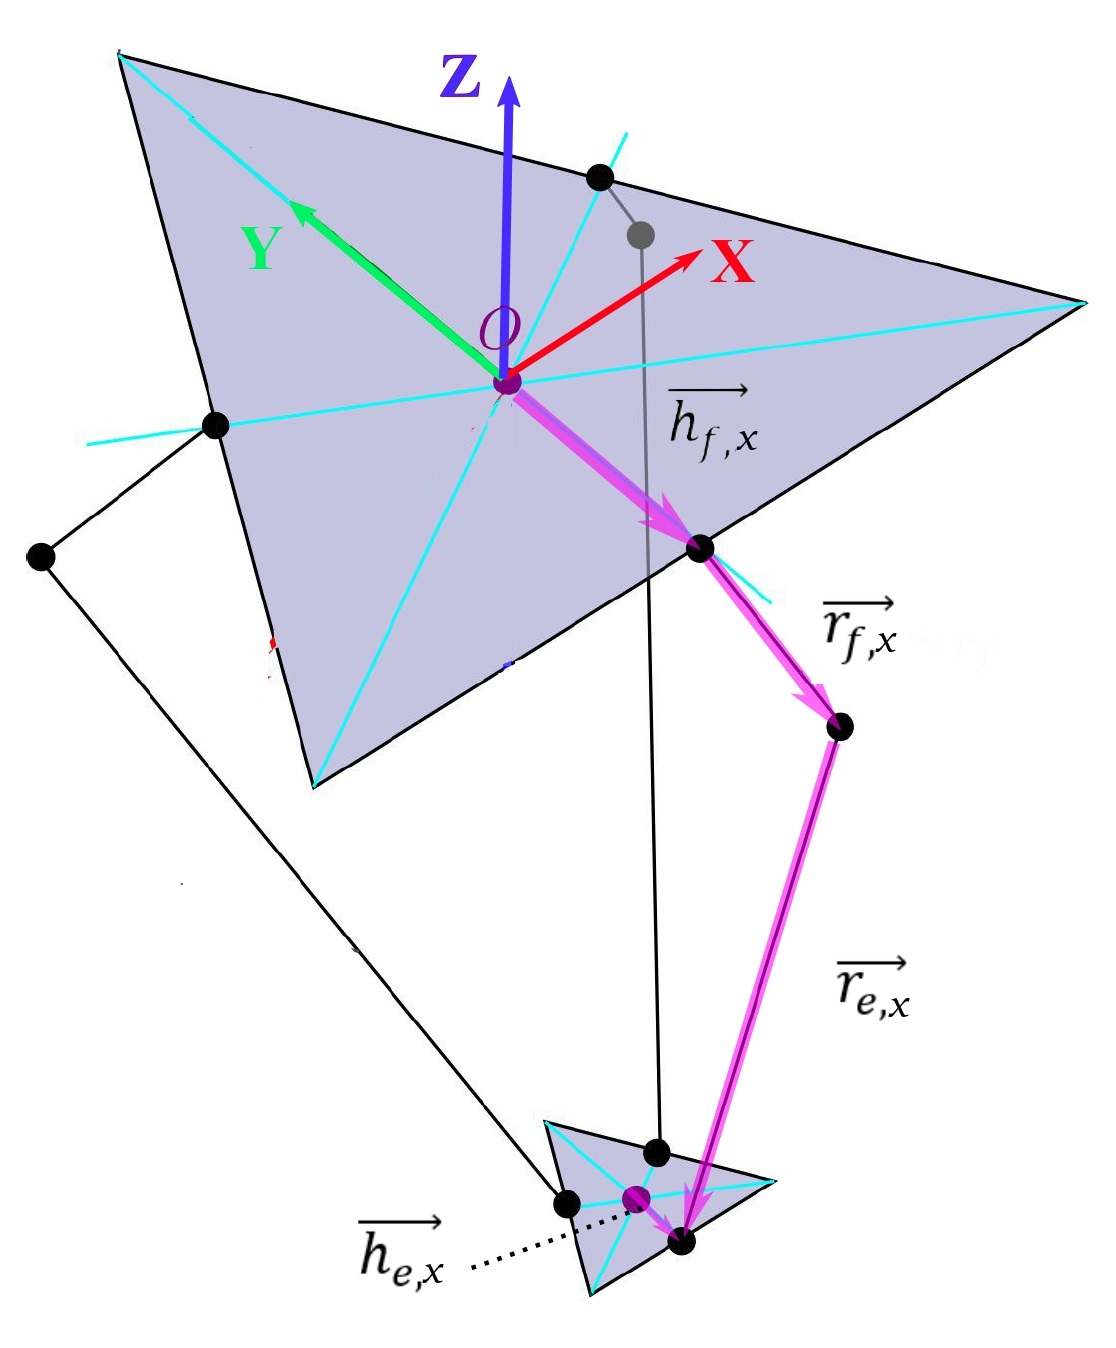
\includegraphics[width=0.7\linewidth]{Main/Chapter4/Images4/DIBUJO16.jpg}
            \caption{Caption}
            \label{fig:ANEXO_MA_C_POS_4}
        \end{figure}

        Se tiene conocimiento de las posiciones de todos los puntos sobre el efector, a causa de que se sabe posición del centroide del efector final  $E_{0} \left( x_{0},y_{0},z_{0} \right)$, la base fija es paralela al efector y además estas dos últimas partes mecánicas mencionadas tienen la misma orientación. Por lo tanto, se conocen las coordenadas de las juntas esféricas  $E_{i}$  que unen los antebrazos con el efector y a su vez los vectores $\overrightarrow{h_{e,x}}$ que representan la posición de las juntas esféricas  $E_{i}$ con respecto al centroide del efector.
        
        Con respecto a los vectores $\overrightarrow{r_{e,x}}$ , que representa los antebrazos, solo se conoce el punto final $E_{i}$ , que coincide con las posiciones de cada junta esférica unida al efector. Entonces, la orientación de cada vector  $\overrightarrow{r_{e,x}}$  , en cada uno de las 3 cadenas, está restringida por esferas con centros en las juntas esféricas $E_{i}$  con radio equivalente al largo del antebrazo $r_{e}$.
             \newpage

        En cuanto a los vectores $\overrightarrow{r_{f,x}}$  solo se conocen sus puntos iniciales $F_{i}$, que coinciden con la posición de cada actuador $i= \{ 1,2,3 \}$, sobre la base fija. Por otro lado, los actuadores son simplificados como juntas revolutas, por ende, restringen a cada uno de los vectores  $\overrightarrow{r_{f,x}}$ a moverse en un plano que contiene un punto en la posición del actuador  $F_{i}$ y un vector  $\overrightarrow{h_{f,x}}$. Las restricciones anteriores traen como consecuencia que las coordenadas de los puntos finales de vector  $\overrightarrow{r_{f,x}}$, es decir su extremo, estén sobre circunferencias Como se aprecia en la figura \ref{fig:ANEXO_MA_C_POS_4}.
        
        Finalmente, para obtener los ángulos de los actuadores  $\left(  \theta _{1}, \theta _{2}, \theta _{3} \right)$  , se calcula las intersecciónes\ entre las circunferencias formadas por el punto final de   $\overrightarrow{r_{f,x}}$  (con centro en  $F_{i}$ y de radio  $r_{f}$) y la esfera formada por el vector  $\overrightarrow{r_{e,x}}$ (con centro en  $E_{i}$ y de radio $r_{e}$) para cada cadena cinemática  $i= \{ 1,2,3 \}$. Esta intersección no es más que la junta esférica  $J_{i}$, recordando que la función de estas es unir los brazos con los antebrazos. Una vez obtenida la posición de las 3 juntas $J_{i}$, con álgebra simple se pueden obtener los valores de los ángulos $\left(  \theta _{1}, \theta _{2}, \theta _{3} \right)$.
        
        Como antes se ha mencionado, el primer paso para encontrar la configuración del espacio articular  $\left(  \theta _{1}, \theta _{2}, \theta _{3} \right)  $ es calcular las posiciones de las juntas $J_{i}$. Se empieza por la junta  $J_{1}$ que esta sobre el plano $YZ$ de nuestro sistema de referencia local. Se puede captar en la figura \ref{fig:ANEXO_MA_C_POS_5} que la intersección de la esfera y el plano $YZ$ es una circunferencia con centro en el punto $E^{'}_{1}$ y de radio $\overline{E^{'}_{1}J_{1}}$ . El punto $E^{'}_{1}$ es la proyección de  $E_{1}$  en el plano $YZ$.
        
        \begin{figure}[htb]
            \centering
            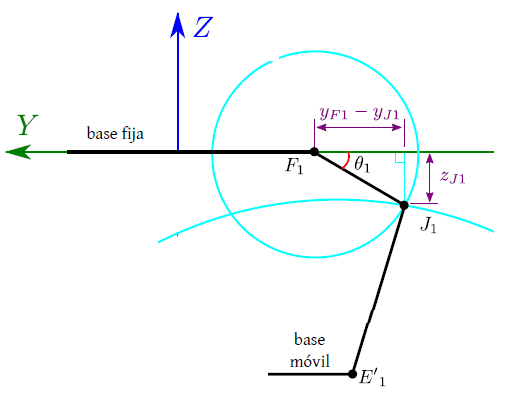
\includegraphics[width=0.9\linewidth]{Main/Chapter4/Images4/DIBUJOA11.png}
            \caption{Caption}
            \label{fig:ANEXO_MA_C_POS_5}
        \end{figure}
     
     \newpage

        El punto  $E_{1}$  que se usa para determinar el centro de la circunferencia $E'_{1}$  gracias a su proyección en el plano $YZ$, se calcula a partir de geometría simple de un triángulo equilátero de lado $e$ y de posición del centroide  $E_{0} \left( x_{0},y_{0},z_{0} \right)$  equivalente a la del efector final:
        
        \vspace{-1em}
        \begin{align*}
            &E_0E_1=\frac{e}{2}tan30=\frac{e}{2\sqrt{3}}\\
            &E_{1} \left( x_{0},y_{0}-\frac{e}{2\sqrt{3}},z_{0} \right) \Longrightarrow E'_{1} \left( 0,y_{0}-\frac{e}{2\sqrt{3}},z_{0} \right)
        \end{align*}


        El radio  $\overline{E^{'}_{1}J_{1}}$ de la circunferencia formada por la proyección del antebrazo en el plano $YZ$, se puede calcular por medio del teorema de pitagoras donde:
        
        \begin{align*}
            &E_1E'_1=x_0\\
            &\Longrightarrow E'_1J_1=\sqrt{E_1{J_1}^{2} - E_1{E'_1}^{2}} = \sqrt{{r_e}^{2}-{x_0}^{2}}
        \end{align*}
        
        
        \begin{figure}[htb]
            \centering
            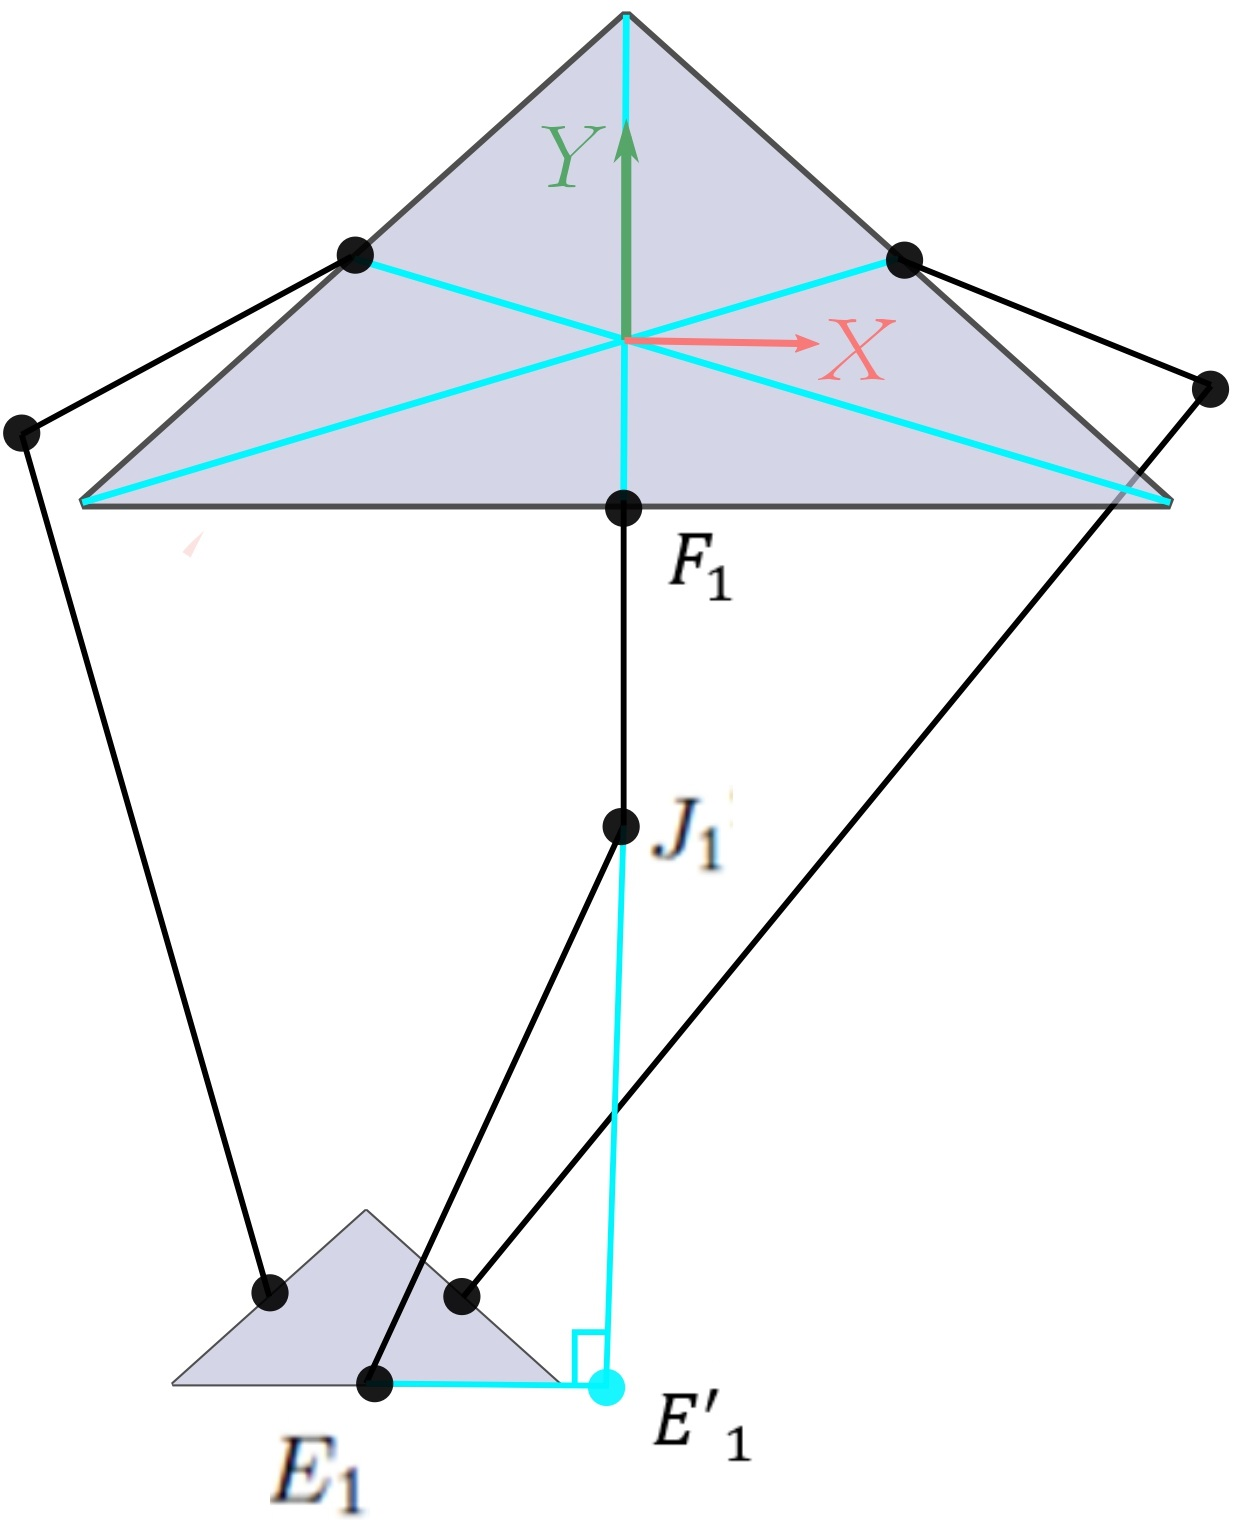
\includegraphics[width=0.7\linewidth]{Main/Chapter4/Images4/DIBUJO12.JPG}
            \caption{Caption}
            \label{fig:ANEXO_MA_C_POS_7}
        \end{figure}      
        
     \newpage
         
       Resumiendo todo lo anterior, los centros de las circunferencias que intersectan la junta esférica $J_{1}$ son:
        \begin{center}
        \renewcommand{\arraystretch}{3.0}
        
            \begin{table}[H]
            \centering
            \begin{tabular}{c c } 
                 \hline
                 \textbf{Centros esferas}  & \textbf{Radio} \\ [0.1ex] 
                 \hline\hline
                         $\left(y_1,z_1\right)$ =
                        $F_1\left(y_{F_1}\,z_{F_1}\right)=\left(-\frac{f}{2\sqrt{3}},0\right)$\textit{} & 
                                                 $r_f$  \\ 
                \hline
                          $(y_2,z_2)$=
                          ${E^'}_{1}$ $(y_{{E^'}_1}$ $z_{{E^'}_1}$ $)=(y_0-\frac{e}{2\sqrt{3}},z_0)$ &
                          $r_2=\sqrt{{r_e}^2-{x_o}^2}$ \\
                \hline
            \end{tabular}
            \caption{Referencias del dibujo}
            \label{tab:anexo_tabla_4}
            \end{table}
        \end{center}

       Ecuaciones cartesianas de las circunferencias son:
        \begin{equation*}
            \left\{ \begin{array}{c}
        	 \left( y-y_{1} \right) ^{2} + \left( z-z_{1} \right) ^{2}= r_{f}^{2}~\\
        	 \left( y-y_{2} \right) ^{2} + \left( z-z_{2} \right) ^{2}=r_{e}^{2}-x_{o}^{2}\\
        	\end{array}\right.
        \end{equation*}
        
        Desarrollando las ecuaciones anteriores y reordenando:
        \begin{equation*}
         \left\{ \begin{array}{c}
        	y^{2}+z^{2}-2yy_{1}-2zz_{1}= r_{f}^{2}-y_{1}^{2}-z_{1}^{2} ~ \left( 1 \right) \\
        	y^{2}+z^{2}-2yy_{2}-2zz_{2}=~ r_{e}^{2}-x_{o}^{2}-y_{2}^{2}-z_{2}^{2}  ~\left( 2 \right) \\
        	\end{array}\right.
        \end{equation*}
        
        Restando $(1)-(2)$
        
        \begin{equation*}
         -2y \left( y_{1}-y_{2} \right) -2z \left( z_{1}-z_{2} \right) = r_{f}^{2}-y_{1}^{2}-z_{1}^{2}- r_{e}^{2}+x_{o}^{2}+y_{2}^{2}+z_{2}^{2} 
        \end{equation*}
        
        Despejando $z$ en función de $y$:
        
        \begin{equation*}
         z=\frac{- \left( y_{1}-y_{2} \right) }{ \left( z_{1}-z_{2} \right) }\ast y+ \frac{r_{f}^{2}-y_{1}^{2}-z_{1}^{2}- r_{e}^{2}+x_{o}^{2}+y_{2}^{2}+z_{2}^{2}}{-2 \left( z_{1}-z_{2} \right)}
        \end{equation*}
        
        Donde:  
        \begin{align*}
             z&=a+by ~\left( 3 \right)\\
             b&=\frac{- \left( y_{1}-y_{2} \right) }{ \left( z_{1}-z_{2} \right) }~\\
             a&= \frac{r_{f}^{2}-y_{1}^{2}-z_{1}^{2}- r_{e}^{2}+x_{o}^{2}+y_{2}^{2}+z_{2}^{2}}{-2 \left( z_{1}-z_{2} \right) } \\ 
        \end{align*}
        
                \newpage

        Reemplazando  $z_{1}=0$, $y_{2}=y_{0}-\frac{e}{2\sqrt[]{3}}$  , $ ~y_{1}=-\frac{f}{2\sqrt[]{3}}$ :
        
        \begin{align*}
         b&=\frac{ \left( y_{1}-y_{2} \right) }{z_{2}}~ \\ 
         a&= \frac{x_{o}^{2}+y_{2}^{2}+z_{0}^{2}+r_{f}^{2}- r_{e}^{2}~-y_{1}^{2}}{2z_{0}} \\
         \Longrightarrow ~ a&= \frac{x_{o}^{2}+ \left( y_{0}-\frac{e}{2\sqrt[]{3}} \right) ^{2}+z_{0}^{2}+r_{f}^{2}- r_{e}^{2}~- \left( -\frac{f}{2\sqrt[]{3}} \right) ^{2}}{2z_{0}}
        \end{align*}
        
        Reemplazando la ecuación $(3)$ en $(1)$:
        
        \begin{equation*}
         \left( y-y_{1} \right) ^{2} + \left[  \left( a+by \right)  -z_{1} \right] ^{2}= r_{f}^{2} 
        \end{equation*}
        
        Desarrollando la ecuación anterior:
        
        \begin{align*}
         &\left( y^{2}-2yy_{1}+y_{1}^{2} \right) + \left( b^{2}y^{2}+2aby+a^{2} \right) -2 \left( a+by \right) z_{1}+ z_{1}^{2}=~r_{f}^{2}~\\
         \Longrightarrow ~~  & \left( b^{2}+1 \right) y^{2}+ \left( -2y_{1}+2ab \right) y + \left( y_{1}^{2}+a^{2}-r_{f}^{2} \right) +z_{1} \left( -2 \left( a+by \right) +z_{1}~ \right) =0~  \left( 4 \right)
        \end{align*}
        
        La solución y para la ecuación cuadrática $(4)$ está dada por:
        
        \begin{equation*}
             y= \frac{- \left( 2ab-2y_{1} \right)   \pm \sqrt[]{d}}{2 \left( b^{2}+1 \right) }
        \end{equation*}
        
        Se aprecian dos soluciones, donde se elige la $y=\frac{- \left( 2ab-2y_{1} \right) -\sqrt[]{d}}{2 \left( b^{2}+1 \right) }$ para que el ángulo entre el brazo y el antebrazo no exceda los 180$ ^{\circ} $.
        
        El discriminante $d$ es:
        
        \begin{equation*}
             d= \left( 2ab-2y_{1} \right) ^{2}-4\ast \left( b^{2}+1 \right) \ast \left[  \left( y_{1}^{2}+a^{2}-r_{f}^{2} \right) +z_{1}\ast \left( -2 \left( a+by \right) +z_{1}\right)  \right]
        \end{equation*}
        
        Reemplazando $z_{1}=0$ y reordenando:
        
        \begin{align*}
         d&= \left( 2ab-2y_{1} \right) ^{2}-4\ast \left( b^{2}+1 \right) \ast \left( y_{1}^{2}+a^{2}-r_{f}^{2} \right) \\
         \Longrightarrow d&=4 \left[ ~ \left( ab-y_{1} \right) ^{2}- \left( b^{2}+1 \right) \ast \left( y_{1}^{2}+a^{2}-r_{f}^{2} \right)  \right]  \\
         \Longrightarrow d&=4 \left[  \left( ~a^{2}b^{2}-2aby_{1}+~y_{1}^{2} \right) + \left( -b^{2}y_{1}^{2}-b^{2}a^{2}+b^{2}r_{f}^{2} \right) - \left( y_{1}^{2}+a^{2}-r_{f}^{2} \right)  \right]  \\
         \Longrightarrow d&=4 \left[ -a^{2}-2aby_{1}-b^{2}y_{1}^{2}+b^{2}r_{f}^{2}+r_{f}^{2} \right]  \\
         \Longrightarrow d&=4 \left[ - \left( a+by_{1} \right) ^{2}+ \left( b^{2}+1 \right) r_{f}^{2} \right]  \\ 
        \end{align*}
        
        \newpage
        
        Por lo tanto, la solución y para el sistema de ecuaciones de las circunferencias es:
        
        \begin{align*}
         y&= \frac{- \left( 2ab-2y_{1} \right) -\sqrt[]{4 \left[ - \left( a+by_{1} \right) ^{2}+ \left( b^{2}+1 \right) r_{f}^{2} \right] }}{2 \left( b^{2}+1 \right) } \\
         \Longrightarrow y&= \frac{ \left( y_{1}-ab \right) -\sqrt[]{ \left[ - \left( a+by_{1} \right) ^{2}+ \left( b^{2}+1 \right) r_{f}^{2} \right] }}{ \left( b^{2}+1 \right) } \\ 
        \end{align*}
        
        Por lo tanto, la solución del sistema de ecuaciones es:

        \begin{equation*}
         J_{1}= \left( x_{J_{1}},y_{J_{1}},z_{J_{1}} \right) = \left( 0,y,a+by \right) 
        \end{equation*}
        
        \begin{equation*}
         J_{1}= \left( 0,\frac{ \left( y_{1}-ab \right) -\sqrt[]{ \left[  \left( a+by_{1} \right) ^{2}+ \left( b^{2}+1 \right) r_{f}^{2} \right] }}{ \left( b^{2}+1 \right) },a+b\frac{ \left( y_{1}-ab \right) -\sqrt[]{ \left[  \left( a+by_{1} \right) ^{2}+ \left( b^{2}+1 \right) r_{f}^{2} \right] }}{ \left( b^{2}+1 \right) } \right)
        \end{equation*}
        
        Finalmente, se determina el ángulo $\theta _{1}$ por medio del triángulo rectángulo formado en el brazo y la proyección del mismo en el plano $XY$, como se ilustra en la figura \ref{fig:ANEXO_MA_C_POS_5}:
        

        \begin{equation*}
         \theta _{1}=\arctan  \left( ~\frac{z_{J_{1}}}{y_{F_{1}}-y_{J_{1}}} \right)  
        \end{equation*}

        
        Donde  $y_{F_{1}}$ se obtiene de la geometría básica que tiene la base fija (figura \ref{fig:ANEXO_MA_C_POS_9}):

        \begin{equation*}
            F_1(0,-\frac{f}{2\sqrt{3}},0)
        \end{equation*}
        
        \begin{figure}[htb]
            \centering
            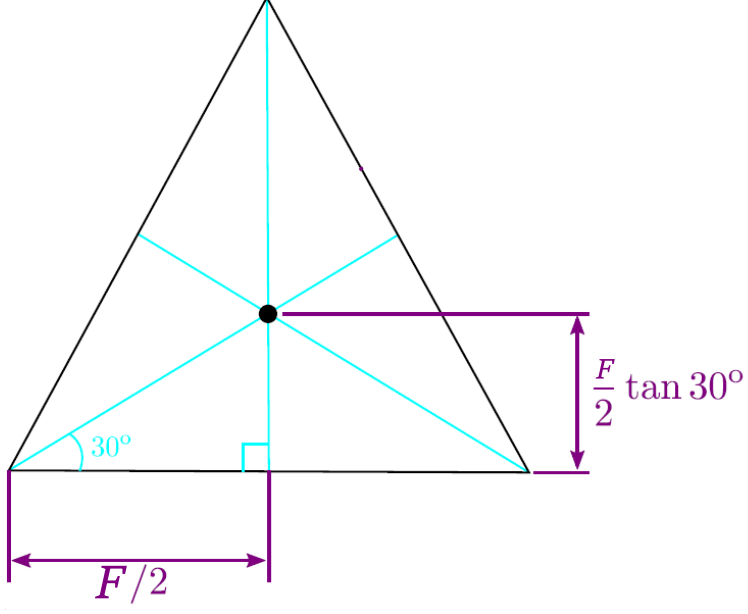
\includegraphics[width=0.5\linewidth]{Main/Chapter4/Images4/DIBUJO15.PNG}
            \caption{Caption}
            \label{fig:ANEXO_MA_C_POS_9}
        \end{figure}
        
        \newpage
        
        Aprovechando la simetría del robot delta, se utiliza el mismo método empleado en la solución de  $\theta _{1}$  para los ángulos  $\theta _{2}$  y  $\theta _{3}$ . Para calcularlos, se utilizan matrices de rotación con un ángulo de rotación de 120$ ^{\circ} $  para la cadena cinemática con el actuador 2 y de 240$ ^{\circ} $  para la cadena cinemática con el actuador 3. Estas matrices giran el sistema de referencia local en 120$ ^{\circ} $  y 240$ ^{\circ} $  grados como se observa en la figura \ref{fig:ANEXO_MA_C_POS_10}:
        
        \begin{figure}[htb]
            \centering
            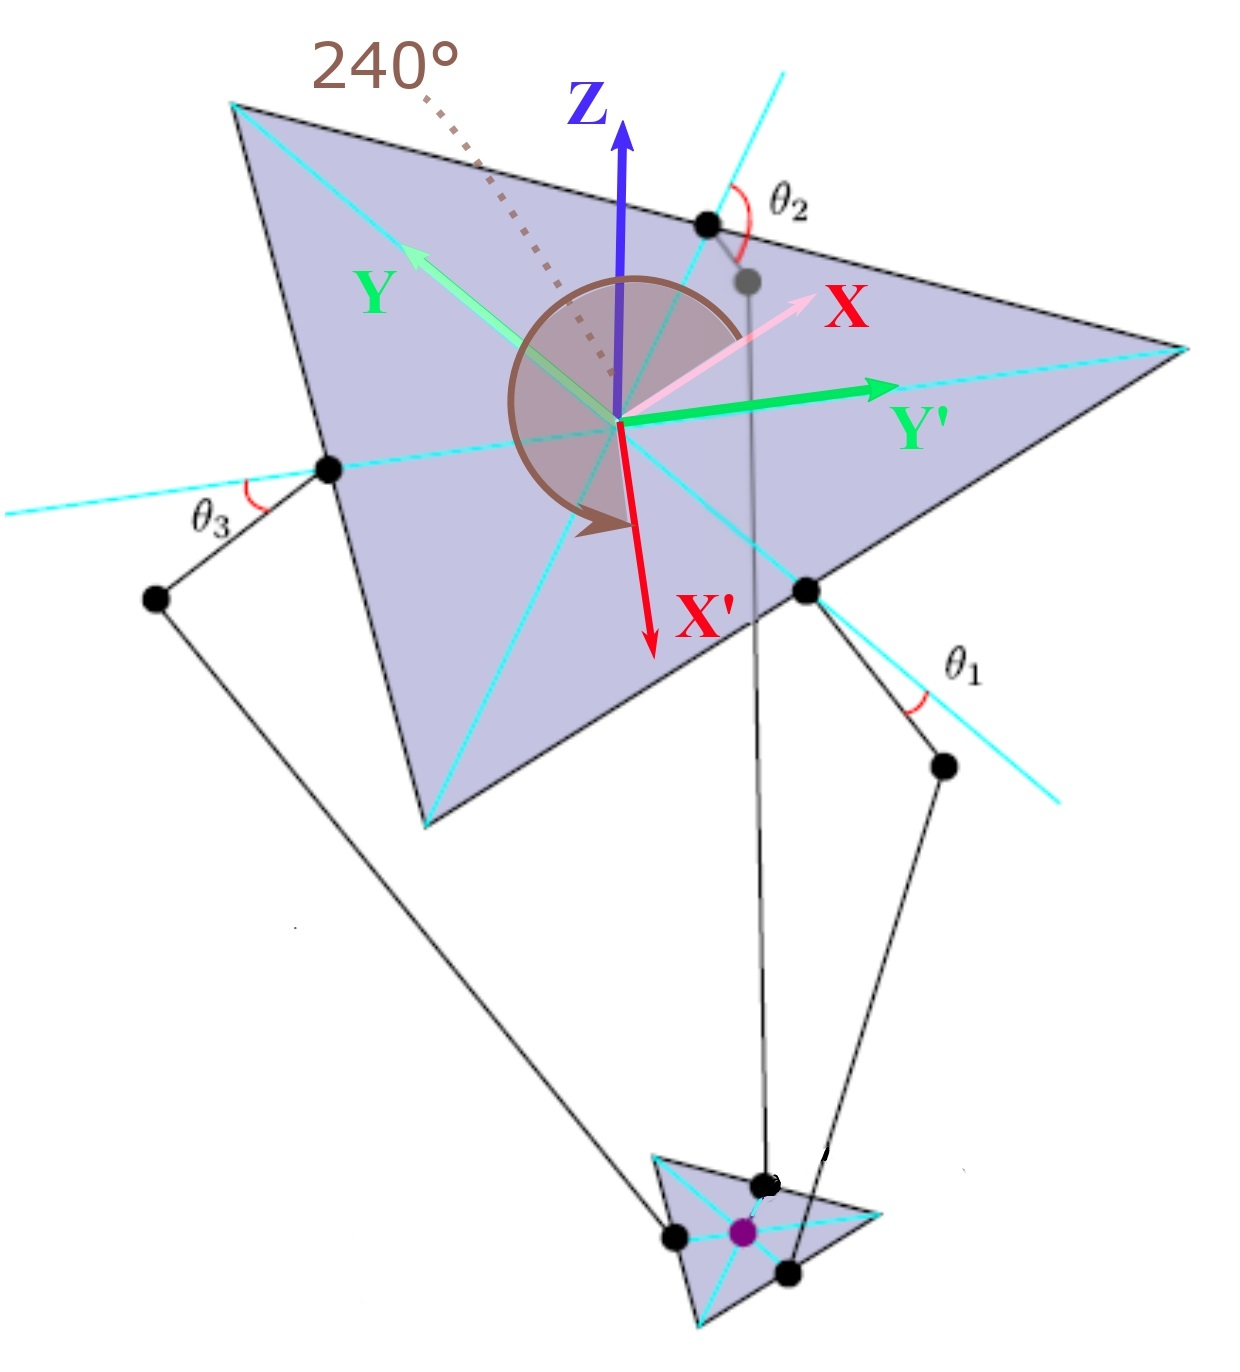
\includegraphics[width=0.9\linewidth]{Main/Chapter4/Images4/DIBUJO17.jpg}
            \caption{Caption}
            \label{fig:ANEXO_MA_C_POS_10}
        \end{figure}
     
     \newpage
        
        
    \subsection{Modelación cinemática de velocidad}\label{anexomodelacionvelocidadmetodoa}
            \subsubsection{Vectorización y ángulos de juntas}
            
        La figura \ref{f:Cap4_Metodo_A_Modelacion_Cinematica_Posicion_8} define los ángulos de articulación asociados con la extremidad  $i$, donde  $\overrightarrow{p}$  es el vector de posición del centroide de la plataforma móvil, $\theta _{1i}$  se mide desde el eje $x_{i}$  hasta $\overrightarrow{A_{i}B_{i}}$ ,$\theta _{2i}$  se define desde la línea extendida de $\overrightarrow{A_{i}B_{i}}$  hasta la línea definida por la intersección del plano del paralelogramo y el plano $x_{i}-z_{i}$ y $\theta _{3i}$  se mide desde la dirección $y_{i}$ hasta $\overrightarrow{B_{i}C_{i}}$ . En general, hay 9 ángulos articulares, $\theta _{1i}$, $\theta _{2i}$ y $\theta _{3i}$ para $i= \{  1, 2, 3 \}$, asociados con el manipulador. Los ángulos de los actuadores son $\theta _{11}$ ,$\theta _{21}$ y $\theta _{31}$ .
        
        Se puede escribir una ecuación de cierre de bucle para cada extremidad vectorialmente:
        
        \begin{equation}
             \overrightarrow{A_{i}B_{i}}+ \overrightarrow{B_{i}C_{i}}~~ =\overrightarrow{OP}~ +\overrightarrow{~PC_{i}} -\overrightarrow{OA_{i}~}
             \label{eq:modelacion_cine_vel_metodoa_anexo_1}
        \end{equation}
        
        Reescribiendo \ref{eq:modelacion_cine_vel_metodoa_anexo_1} en el marco de coordenadas  $A_{i}$ –    $x_{i}y_{i}z_{i}$ conduce a la siguiente representación matricial:
        
        \begin{equation}
                 a \left[ \begin{matrix}
                cos~ \theta _{1i}\\
                0\\
                sin~ \theta _{1i}\\
                \end{matrix}
                 \right] +b \left[ \begin{matrix}
                sin~ \theta _{3i}cos⁡ \left(  \theta _{1i}+ \theta _{2i} \right) \\
                cos~ \theta _{3i}\\
                sin~ \theta _{3i}sin \left(  \theta _{1i}+ \theta _{2i} \right) \\
                \end{matrix}
                 \right] = \left[ \begin{matrix}
                c_{xi}\\
                c_{yi}\\
                c_{zi}\\
                \end{matrix} \right] 
                \label{eq:modelacion_cine_vel_metodoa_anexo_2}
        \end{equation}
        
        \begin{equation}
                    \left[ \begin{matrix}
                    c_{xi}\\
                    c_{yi}\\
                    c_{zi}\\
                    \end{matrix}
                     \right] = \left[ \begin{matrix}
                    \cos  \phi _{i}  &  \sin  \phi _{i}  &  0\\
                    -sin \phi _{i}  &  \cos  \phi _{i}  &  0\\
                    0  &  0  &  1\\
                    \end{matrix}
                     \right]  \left[ \begin{matrix}
                    p_{x}\\
                    p_{y}\\
                    p_{z}\\
                    \end{matrix}
                     \right] +  \left[ \begin{matrix}
                    h\\
                    0\\
                    0\\
                    \end{matrix}
                     \right] - \left[ \begin{matrix}
                    r\\
                    0\\
                    0\\
                    \end{matrix}
                     \right] 
                \label{eq:modelacion_cine_vel_metodoa_anexo_3}
        \end{equation}

        \begin{figure}[htb]
            \centering
            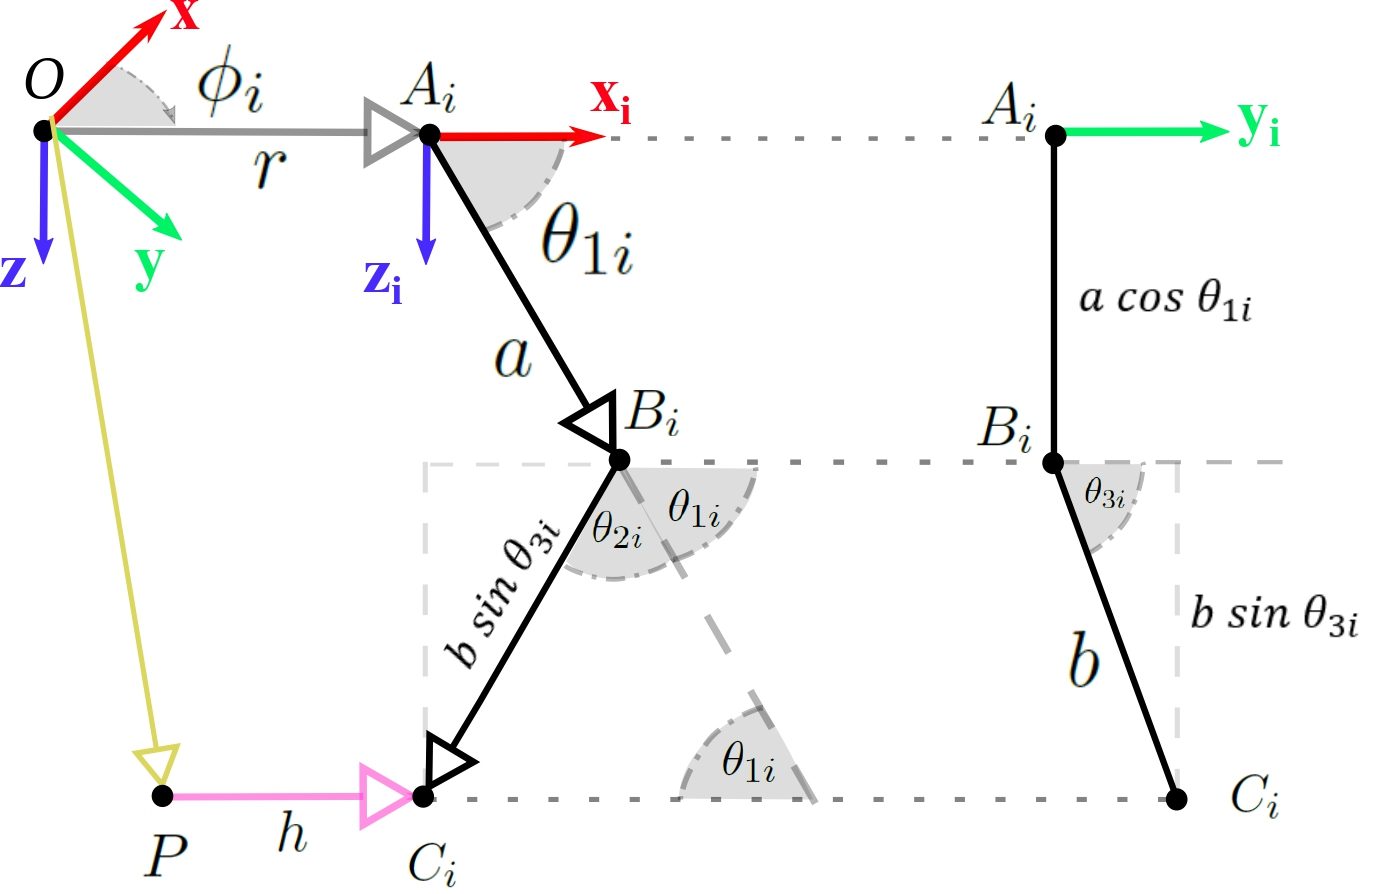
\includegraphics[width=0.9\linewidth]{Main/Chapter4/Images4/DIBUJO22.jpg}
            \caption{Caption}
            \label{fig:ANEXO_MA_C_vel_1}
        \end{figure}
     
        \newpage


        La figura \ref{fig:ANEXO_MA_C_vel_1} denota la posición del punto  $C_{i}$  en relación con el marco de coordenadas  $A_{i}$ – $x_{i}y_{i}z_{i}$ ,$a$  y  $b$ son las longitudes de los enlaces $\overrightarrow{A_{i}B_{i}}$ , y  $\overrightarrow{B_{i}C_{i}}$  respectivamente y $\overrightarrow{p}= \left[ p_{x},p_{y},p_{z} \right] ^{T}$  es el vector de posición del punto $P$   relativo al sistema de coordenadas $O$ – $xyz$.
        
        El ángulo $\theta _{3i}$  se calcula resolviendo la segunda fila de la ecuación \ref{eq:modelacion_cine_vel_metodoa_anexo_2}:

        \begin{equation}
            \theta _{3i}= \cos ^{-1}\frac{c_{yi}}{b} 
            \label{eq:modelacion_cine_vel_metodoa_anexo_3}
        \end{equation}
        
        Con  $\theta _{3i}$  determinado, se genera una ecuación con $\theta _{2i}$ como la única incógnita, sumando los cuadrados de  $c_{xi}$ ,  $c_{yi}$  y  $c_{zi}$ en la ecuación \ref{eq:modelacion_cine_vel_metodoa_anexo_2} aplicando la norma a los vectores:
        \vspace{-1em}
        
      \begin{equation*}
                      &\left \Vert a
            \left[ \begin{matrix}
            cos~ \theta _{1i}\\
            0\\
            sin~ \theta _{1i}\\
            \end{matrix}\right] +b \left[ \begin{matrix}
            sin~ \theta _{3i} cos⁡ \left(  \theta _{1i}+ \theta _{2i} \right) \\
            cos~ \theta _{3i}\\
            sin~ \theta _{3i}sin \left(  \theta _{1i}+ \theta _{2i} \right) \\
            \end{matrix}
             \right] ~~ \right \Vert =~~ \left \Vert ~~~ \left[ \begin{matrix}
            c_{xi}\\
            c_{yi}\\
            c_{zi}\\
            \end{matrix}
             \right] ~~~ \right \Vert \\
      \end{equation*}  
              \vspace{-1em}
     \begin{align*}
             \Longrightarrow & \left( a cos~ \theta _{1i}+b sin~ \theta _{3i}~cos⁡ \left(  \theta _{1i}+ \theta _{2i} \right)  \right) ^{2}+\\
              &\left( b cos~ \theta _{3i} \right) ^{2}+ \left( a sin~ \theta _{1i}+b sin~ \theta _{3i}sin \left(  \theta _{1i}+ \theta _{2i} \right)  \right) ^{2} = c_{xi}^{2}+c_{yi}^{2}+c_{zi}^{2}\\
             \Longrightarrow &  \left[ a^{2}cos^{2}\theta _{1i}+\2ab cos~ \theta _{1i}sin~ \theta _{3i}\cos  \left(  \theta _{1i}+ \theta _{2i} \right) +b^{2}sin ^{2}~ \theta _{3i} cos ^{2}⁡ \left(  \theta _{1i}+ \theta _{2i} \right) \right] +\\
             &\left[ b^{2}~cos^{2} \theta _{3i} \right] + \left[ a^{2}~sin^{2} \theta _{1i}+2ab~sin~ \theta _{1i}sin~ \theta _{3i}sin \left(  \theta _{1i}+ \theta _{2i} \right) +b^{2}sin^{2}  \theta _{3i} sin^{2}  \left(  \theta _{1i}+ \theta _{2i} \right) \right]=\\
             &c_{xi}^{2}+c_{yi}^{2}+c_{zi}^{2}\\
             \Longrightarrow & a^{2} \left( cos^{2} \theta _{1i}+~sin^{2} \theta _{1i} \right) +b^{2}sin^{2} ~ \theta _{3i} \left( \cos^{2}   \left(  \theta _{1i}+ \theta _{2i} \right)+\sin^{2}   \left(  \theta _{1i}+ \theta _{2i} \right)\right) +\\
             &2 ab sin~ \theta _{3i} \left( ~cos~ \theta _{1i}\cos  \left(  \theta _{1i}+ \theta _{2i} \right) +sin~ \theta _{1i}\sin  \left(  \theta _{1i}+ \theta _{2i} \right)  \right) +b^{2}~cos^{2} \theta _{3i}= c_{xi}^{2}+c_{yi}^{2}+c_{zi}^{2}
        \end{align*}
        
        Utilizando las siguientes propiedades trigonométricas:
        \begin{gather*}
            \cos^{2}~ \theta _{1i}+~sin^{2}~ \theta _{1i}=1\\
            \cos^{2}  \left(  \theta _{1i}+ \theta _{2i} \right)+\sin ^{2} \left(  \theta _{1i}+ \theta _{2i} \right) =1 \\
            \cos \theta _{1i}\cos  \left(  \theta _{1i}+ \theta _{2i} \right) +sin~ \theta _{1i}sin \left(  \theta _{1i}+ \theta _{2i} \right) =cos⁡  \left(  \theta _{1i}- \left(  \theta _{1i}+ \theta _{2i} \right)  \right) = cos⁡  \left(  \theta _{2i} \right)
        \end{gather*}

        Reemplazando:
        \begin{equation*}
         \Longrightarrow a^{2}+b^{2}sin^{2} ~ \theta _{3i}+ 2 ab sin~ \theta _{3i}\cos  \theta _{2i}+b^{2}~cos^{2} ~ \theta _{3i}= c_{xi}^{2}+c_{yi}^{2}+c_{zi}^{2} 
        \end{equation*}
        
        Donde se sabe que:
        \begin{equation*}
            \left( sin^{2}~ \theta _{3i}+~cos^{2} \theta _{3i} \right) =1
        \end{equation*}
        
        Entonces:
        \begin{equation*}
            a^{2}+b^{2}+ 2 ab sin~ \theta _{3i}\cos  \theta _{2i}+b^{2}= c_{xi}^{2}+c_{yi}^{2}+c_{zi}^{2}
        \end{equation*}
        
        Despejando  $\theta _{2i}$:
                \vspace{-0.2em}
        \begin{equation}
          \theta _{2i}=\cos ^{-1} \left( \frac{c_{xi}^{2}+c_{yi}^{2}+c_{zi}^{2}- a^{2}-b^{2}~}{2 ab sin~ \theta _{3i}} \right) 
        \end{equation}
        
        Con  $\theta _{3i}$  y  $\theta _{2i}$  determinados, solo queda un par de ecuaciones con $\theta _{1i}$  como la única incógnita que desde la ecuación \ref{eq:modelacion_cine_vel_metodoa_anexo_2}. Por lo tanto, es posible resolver el valor de $ \theta _{1i}$.

\newpage


        \subsubsection{Jacobiano}
            Con referencia a la figura \ref{fig:ANEXO_MA_C_vel_1}, una ecuación de cierre de bucle para una extremidad $i$ sistema de referencia $A_{i}$ – $ x_{i}y_{i}z_{i}$  se puede escribir como:
            
            \begin{equation}
                 \overrightarrow{OP}+\overrightarrow{~PC_{i}} =\overrightarrow{OA_{i}}+\overrightarrow{A_{i}B_{i}}+\overrightarrow{B_{i}C_{i}}
            \label{eq:jac_met_a_anex_1}
            \end{equation}
            
            Al diferenciar vectorialmente la ecuación \ref{eq:jac_met_a_anex_1} con respecto a el tiempo:
            
            \begin{equation*}
                 \dot{\overrightarrow{OP}}+\dot{\overrightarrow{~PC_{i}}}= \dot{\overrightarrow{OA_{i}}}+ \dot{\overrightarrow{A_{i}B_{i}}}+ \dot{\overrightarrow{B_{i}C_{i}}} 
            \end{equation*}
            
            Donde  $\dot{\overrightarrow{~PC_{i}}}= \dot{\overrightarrow{OA_{i}}}=0$ , entonces:
            
            \begin{equation}
                 \overrightarrow{v_{p}}= \overrightarrow{ \omega _{1i}}~\times~~\overrightarrow{a_{i}}+  \overrightarrow{ \omega _{2i}}~\times~\overrightarrow{b_{i}}
            \label{eq:jac_met_a_anex_2}
            \end{equation}
            
            Donde  $ \overrightarrow{v_{p}}= \left[ v_{px},v_{py},v_{pz} \right] ^{T}$ es la velocidad lineal de la plataforma móvil, $\overrightarrow{a_{i}}= \overrightarrow{A_{i}B_{i}}$, $ \overrightarrow{b_{i}}=\overrightarrow{~B_{i}C_{i}}$  y   $\overrightarrow{ \omega _{ji}}$  es la velocidad angular del eslabón $j$ de la cadena cinemática $i$. Para eliminar $\omega _{2i}$  es necesario hacer un producto punto en ambos lados de la ecuación \ref{eq:jac_met_a_anex_2} por un vector unitario  $ \widehat{b_{i}} $ . Por lo tanto:
            \vspace{-0.5em}
            \begin{align*}
                 \widehat{b_{i}} \cdot  \overrightarrow{v_{p}}&= \widehat{b_{i}}  \cdot  \left( ~\overrightarrow{ \omega _{1i}}~\times~~\overrightarrow{a_{i}}~~~+  \overrightarrow{ \omega _{2i}}~\times~\overrightarrow{b_{i}} \right) ~~~ \\ 
                 \Longrightarrow ~\widehat{b_{i}}  \cdot  \overrightarrow{v_{p}}&= \widehat{b_{i}}  \cdot  \left( ~\overrightarrow{ \omega _{1i}}~\times~~\overrightarrow{a_{i}}~ \right)  +\widehat{b_{i}}  \cdot  \left( ~\overrightarrow{ \omega _{2i}}~\times~\overrightarrow{b_{i}} \right) ~~~  \\ 
                 \Longrightarrow ~\widehat{b_{i}}  \cdot  \overrightarrow{v_{p}}&= \overrightarrow{ \omega _{1i}} \cdot  \left( ~\overrightarrow{a_{i}}~\times~~\widehat{b_{i}}~ \right)  +\overrightarrow{ \omega _{2i}} \cdot  \left( \overrightarrow{b_{i}}~\times~\widehat{b_{i}}~ \right) ~  \\
                 \Longrightarrow ~\widehat{b_{i}}  \cdot  \overrightarrow{v_{p}}&= \overrightarrow{ \omega _{1i}} \cdot  \left( ~\overrightarrow{a_{i}}~\times~~\widehat{b_{i}} \right) ~  \\
                 \Longrightarrow ~~\widehat{b_{i}} \cdot \overrightarrow{v_{p}}&= \widehat{b_{i}} \cdot  \left( ~\overrightarrow{ \omega _{1i}}~\times~\overrightarrow{a_{i}} \right)
            \end{align*}
            
            Por lo tanto, la igualdad que se utiliza para calcular el jacobiano es: 
            \begin{equation}
                \widehat{b_{i}} \cdot \overrightarrow{v_{p}}&= \widehat{b_{i}} \cdot  \left( ~\overrightarrow{ \omega _{1i}}~\times~\overrightarrow{a_{i}} \right)
                \label{eq:jac_met_a_anex_3}
            \end{equation}
            
            El vector unitario del vector  $\overrightarrow{b_{i}}$ es calculado con la siguiente expresión:
            
            \begin{equation*}
                \widehat{b_{i}}&=\frac{\overrightarrow{b_{i}}}{ \Vert \overrightarrow{b_{i}} \Vert }=\frac{\overrightarrow{b_{i}}}{b}= \left[ \begin{matrix}
                sin~ \theta _{3i}cos⁡ \left(  \theta _{1i}+ \theta _{2i} \right) \\
                cos~ \theta _{3i}\\
                sin~ \theta _{3i}sin \left(  \theta _{1i}+ \theta _{2i} \right) \\
                \end{matrix}
                 \right]  
            \end{equation*}
            
            Al reescribir los vectores de la ecuación \ref{eq:jac_met_a_anex_3} en el marco de coordenadas  $A_{i}$–$x_{i}y_{i}z_{i}$ conduce a:
            
            \begin{align*}
                            \overrightarrow{a_{i}}= a \left[ \begin{matrix}
                cos~ \theta _{1i}\\
                0\\
                sin~ \theta _{1i}\\
                \end{matrix}
                 \right] ;   &             \overrightarrow{b_{i}}=b \left[ \begin{matrix}
                sin~ \theta _{3i}cos⁡ \left(  \theta _{1i}+ \theta _{2i} \right) \\
                cos~ \theta _{3i}\\
                sin~ \theta _{3i}sin \left(  \theta _{1i}+ \theta _{2i} \right) \\
                \end{matrix}\right];           &               \overrightarrow{ \omega _{1i}}= \left[ \begin{matrix}
                0\\
                -\dot{ \theta _{1i}}\\
                0\\
                \end{matrix}
                 \right];&\overrightarrow{v_{p}}= \left[ \begin{matrix}
                v_{px}\cos  \phi _{i}+v_{py}\sin  \phi _{i}\\
                -v_{px}\sin  \phi _{i}+v_{py}\cos  \phi _{i}\\
                v_{pz}\\
                \end{matrix} \right]
            \end{align*}
            
            El signo negativo en la segunda fila de  $\overrightarrow{ \omega _{1i}}$ es solo una cuestión de convención. 

            \newpage
            
            Calculando  $\widehat{b_{i}} \cdot \overrightarrow{v_{p}}$,  sustituyendo los valores $\widehat{b_{i}}$ y  $\overrightarrow{v_{p}}$:

            \begin{align*}
                  \widehat{b_{i}} \cdot \overrightarrow{v_{p}} &= \left[ \begin{matrix}
                    sin~ \theta _{3i}cos⁡ \left(  \theta _{1i}+ \theta _{2i} \right) \\
                    cos~ \theta _{3i}\\
                    sin~ \theta _{3i}sin \left(  \theta _{1i}+ \theta _{2i} \right) \\
                    \end{matrix}
                     \right]  \cdot  \left[ \begin{matrix}
                    v_{px}\cos  \phi _{i}+v_{py}\sin  \phi _{i}\\
                    -v_{px}\sin  \phi _{i}+v_{py}\cos  \phi _{i}\\
                    v_{pz}\\
                    \end{matrix}
                     \right]\\
                 &= \left[  \left( sin~ \theta _{3i}cos⁡ \left(  \theta _{1i}+ \theta _{2i} \right)  \right) \ast \left( v_{px}\cos  \phi _{i}+v_{py}\sin  \phi _{i} \right)  \right] +\\
                 ~~ &\left[  \left( cos~ \theta _{3i} \right) \ast \left( -v_{px}\sin  \phi _{i}+v_{py}\cos  \phi _{i} \right)  \right] +\\
                 ~~~&\left[  \left( sin~ \theta _{3i}sin \left(  \theta _{1i}+ \theta _{2i} \right)  \right) \ast \left( v_{pz} \right)  \right] \\
                 &= \left[ sin~ \theta _{3i}\cos  \left(  \theta _{1i}+ \theta _{2i} \right) \cos  \phi _{i}-cos  \theta _{3i}\sin  \phi _{i} \right] v_{px}+\\
                 ~~~&\left[ sin~ \theta _{3i}\cos  \left(  \theta _{1i}+ \theta _{2i} \right) \sin  \phi _{i}+ cos  \theta _{3i}\cos  \phi _{i} \right] v_{py}+\\ 
                 ~~~&\left[  \left( sin~ \theta _{3i}sin \left(  \theta _{1i}+ \theta _{2i} \right)  \right)  \right] v_{pz} \\
                 &=J_{ix}v_{px}+J_{iy}v_{py}+J_{iz}v_{pz} 
            \end{align*}
            
            Por lo tanto:
            \begin{equation}
                 \widehat{b_{i}} \cdot \overrightarrow{v_{p}} =J_{ix}v_{px}+J_{iy}v_{py}+J_{iz}v_{pz}
                                 \label{eq:jac_met_a_anex_5}
            \end{equation}
            
            Donde:
            \begin{align}
                  J_{ix}&=\cos  \left(  \theta _{1i}+ \theta _{2i} \right) sin~ \theta _{3i}\cos  \phi _{i}-cos  \theta _{3i}\sin  \phi _{i}~\\
                  J_{iy}&=\cos  \left(  \theta _{1i}+ \theta _{2i} \right) sin~ \theta _{3i}\sin  \phi _{i}+ cos  \theta _{3i}\cos  \phi _{i}~ \\
                  J_{iz}&=sin \left(  \theta _{1i}+ \theta _{2i} \right) sin~ \theta _{3i}~ 
                \end{align}
                
                Calculando $\widehat{b_{i}} \cdot  \left( ~\overrightarrow{ \omega _{1i}}~\times~\overrightarrow{a_{i}} \right)$, sustituyendo los valores $\overrightarrow{a_{i}}$, $\widehat{b_{i}}$, $\overrightarrow{ \omega _{1i}}$:
                
                \begin{align*}
                 &\widehat{b_{i}} \cdot  \left( ~\overrightarrow{ \omega _{1i}}~\times~\overrightarrow{a_{i}} \right)= \left[ \begin{matrix}
                sin~ \theta _{3i}cos⁡ \left(  \theta _{1i}+ \theta _{2i} \right) \\
                cos~ \theta _{3i}\\
                sin~ \theta _{3i}sin \left(  \theta _{1i}+ \theta _{2i} \right) \\
                \end{matrix}
                 \right]  \cdot   \left( ~ \left[ \begin{matrix}
                0\\
                -\dot{ \theta _{1i}}\\
                0\\
                \end{matrix}
                 \right] \times a \left[ \begin{matrix}
                cos~ \theta _{1i}\\
                0\\
                sin~ \theta _{1i}\\
                \end{matrix}
                 \right]  \right) \\
                &= \left[ \begin{matrix}
                sin~ \theta _{3i}cos⁡ \left(  \theta _{1i}+ \theta _{2i} \right) \\
                cos~ \theta _{3i}\\
                sin~ \theta _{3i}sin \left(  \theta _{1i}+ \theta _{2i} \right) \\
                \end{matrix}
                 \right]  \cdot  a \left[ \begin{matrix}
                -sin  \theta _{1i}\dot{ \theta _{1i}}\\
                0\\
                cos~ \theta _{1i}\dot{ \theta _{1i}}\\
                \end{matrix}
                 \right] \\
                 &=a~  \left( -sin  \theta _{3i}cos⁡ \left(  \theta _{1i}+ \theta _{2i} \right) sin  \theta _{1i}\dot{ \theta _{1i}} \right) + \left( sin~ \theta _{3i}sin \left(  \theta _{1i}+ \theta _{2i} \right) cos  \theta _{1i}\dot{ \theta _{1i}} \right)  \\
                 &=a~ \dot{ \theta _{1i}}sin~ \theta _{3i} \left( -\cos  \left(  \theta _{1i}+ \theta _{2i} \right) sin~ \theta _{1i}+sin \left(  \theta _{1i}+ \theta _{2i} \right) cos  \theta _{1i} \right) \\
                 &=a~ \dot{ \theta _{1i}}~sin~ \theta _{3i}~ \left( -\cos  \left(  \theta _{1i}+ \theta _{2i} \right) sin~ \theta _{1i}+sin \left(  \theta _{1i}+ \theta _{2i} \right) cos  \theta _{1i} \right) \\
                 &=a~ \dot{ \theta _{1i}}~sin~ \theta _{3i} sin \left(  \theta _{1i}+ \theta _{2i}- \theta _{1i} \right)\\
                 &=a~ \dot{ \theta _{1i}~}sin~ \theta _{3i}~sin \theta _{2i} \\
                 &=a~ \sin  \theta _{2i}~sin~ \theta _{3i}~\dot{ \theta _{1i}}
            \end{align*}
            
            Por lo tanto:
            
            \begin{equation}
                \widehat{b_{i}} \cdot  \left( ~\overrightarrow{ \omega _{1i}}~\times~\overrightarrow{a_{i}} \right)=a~ \sin  \theta _{2i}~sin~ \theta _{3i}~\dot{ \theta _{1i}}
                                \label{eq:jac_met_a_anex_6}
            \end{equation}
            
                        \newpage

           Sustituyendo las ecuaciones \ref{eq:jac_met_a_anex_5} y \ref{eq:jac_met_a_anex_6} en la ecuación \ref{eq:jac_met_a_anex_3}:
            
            \begin{equation}
                J_{ix}v_{px}+J_{iy}v_{py}+J_{iz}v_{pz}=a~\sin  \theta _{2i}~sin~ \theta _{3i}~\dot{ \theta _{1i}}~
            \label{eq:jac_met_a_anex_7}
            \end{equation}

            
            Al expandir la ecuación \ref{eq:jac_met_a_anex_7} para i =1,2,3 se obtienen tres ecuaciones escalares:
            
            \vspace{-0.5cm}
            
            \begin{align*}
             J_{1x}v_{px}+J_{1y}v_{py}+J_{1z}v_{pz}&=a~\sin  \theta _{21}~sin~ \theta _{31}~\dot{ \theta _{11}}~ \\
             J_{2x}v_{px}+J_{2y}v_{py}+J_{2z}v_{pz}&=a~\sin  \theta _{22}~sin~ \theta _{32}~\dot{ \theta _{12}}~ \\
             J_{3x}v_{px}+J_{3y}v_{py}+J_{3z}v_{pz}&=a~\sin  \theta _{23}~sin~ \theta _{33}~\dot{ \theta _{13}}~ \\ 
            \end{align*}
            
                        \vspace{-0.5cm}


            Se ensambla en una forma matricial como:
            
            \begin{equation*}
                 \left[ \begin{matrix}
                J_{1x}  &  J_{1y}  &  J_{1z}\\
                J_{2x}  &  J_{2y}  &  J_{2z}\\
                J_{3x}  &  J_{3y}  &  J_{3z}\\
                \end{matrix}
                 \right]  \left[ \begin{matrix}
                v_{px}\\
                v_{py}\\
                v_{pz}\\
                \end{matrix}
                 \right] = \left[ \begin{matrix}
                a~\sin  \theta _{21}~sin~ \theta _{31}~  &  0  &  0\\
                0  &  a~\sin  \theta _{22}~sin~ \theta _{32}~  &  0\\
                0  &  0  &  a~\sin  \theta _{23}~sin~ \theta _{33}\\
                \end{matrix}
                 \right]  \left[ \begin{matrix}
                \dot{ \theta _{11}}~\\
                \dot{ \theta _{12}}\\
                \dot{ \theta _{13}}~\\
                \end{matrix}
                 \right] 
            \end{equation*}
            
            Se les asignan símbolos las matrices como:
            
            \begin{equation}
                J_{x}v_{p}=J_{ \theta }\dot{ \theta }
            \label{eq:jac_met_a_anex_8}
            \end{equation}
            
            Donde:
            
             \[ J_{ \theta }=  \left[ \begin{matrix}
            J_{1 \theta }~  &  0  &  0\\
            0  &  J_{2 \theta }~~  &  0\\
            0  &  0  &  J_{3 \theta }~\\ 
            \end{matrix}
             \right] ~  ;  J_{x}=\left[ \begin{matrix}
                J_{1x}  &  J_{1y}  &  J_{1z}\\
                J_{2x}  &  J_{2y}  &  J_{2z}\\
                J_{3x}  &  J_{3y}  &  J_{3z}\\
                \end{matrix}
                 \right]  \] 
            
            Asignando subíndices estándar para las 3 cadenas cinemáticas:
            
            \begin{equation}
              J_{i \theta }=a~\sin  \theta _{2i}~sin~ \theta _{3i}~~~,  i= \{ 1,2,3 \}   
            \end{equation}
            
            Manipulando la ecuación anterior algebraicamente:
            
            \begin{equation}
                 v_{p}=J\dot{ \theta }
            \end{equation}
            
            Finalmente, el jacobiano es   $J$  y representa el cambio de las posiciones en el espacio cartesiano de la plataforma móvil respecto al cambio de los ángulos en el espacio articular de los actuadores:
            
            \begin{equation}
                 J= \left[ \begin{matrix}
                \frac{ \partial x}{ \partial  \theta _{1}}  &  \frac{ \partial x}{ \partial  \theta _{2}}  &  \frac{ \partial x}{ \partial  \theta _{3}}\\
                \frac{ \partial y}{ \partial  \theta _{1}}  &  \frac{ \partial y}{ \partial  \theta _{2}}  &  \frac{ \partial y}{ \partial  \theta _{3}}\\
                \frac{ \partial z}{ \partial  \theta _{1}}  &  \frac{ \partial z}{ \partial  \theta _{2}}  &  \frac{ \partial z}{ \partial  \theta _{3}}\\
                \end{matrix}
                 \right]
            \end{equation}
            
           Donde:
           
           \begin{itemize}
               \item { $J=J_{x}^{-1}J_{ \theta }$  es el jacobiano del robot delta}
               \item {$ v_{p}= \left[ v_{px},v_{py},v_{pz} \right] ^{T}$ es la velocidad del del punto $p $ en la plataforma móvil}
               \item {$\dot{ \theta }= \left[ \dot{ \theta _{11}},\dot{ \theta _{12}},\dot{ \theta _{13}}  \right] ^{T}$ es la velocidad angular de los actuadores}
           \end{itemize}
        
            \newpage
            
  \subsection{Modelación Cinemática Aceleración (A)}
            Desde la sección \ref{anexomodelacionvelocidadmetodoa}, modelación cinemática de velocidad, se tiene que:

            \begin{equation}
                J_{x}v_{p}&=J_{ \theta }\dot{ \theta }  \\
                \label{eq:axnexo_metod_a_acel_1}
                        \end{equation}
                        
             \begin{equation*}
                   \left[ \begin{matrix}
                J_{1x}  &  J_{1y}  &  J_{1z}\\
                J_{2x}  &  J_{2y}  &  J_{2z}\\
                J_{3x}  &  J_{3y}  &  J_{3z}\\
                \end{matrix}
                 \right]  \left[ \begin{matrix}
                v_{px}\\
                v_{py}\\
                v_{pz}\\
                \end{matrix}
                 \right] &= \left[ \begin{matrix}
                J_{1 \theta }~  &  0  &  0\\
                0  &  J_{2 \theta }~~  &  0\\
                0  &  0  &  J_{3 \theta }~\\
                \end{matrix}
                 \right] ~ \left[ \begin{matrix}
                \dot{ \theta _{11}}~\\
                \dot{ \theta _{12}}\\
                \dot{ \theta _{13}}~\\
                \end{matrix}
                 \right]   
            \end{equation*}
            
            Derivando matricialmente la ecuación \ref{eq:axnexo_metod_a_acel_1}:
            \begin{align*}
                 \dot{J}_{x}v_{p}+J_{x}\dot{v}_{p}&=\dot{J}_{ \theta }\dot{ \theta }+J_{ \theta }\ddot{ \theta }\\
                 \Longrightarrow \dot{J}_{x}v_{p}+J_{x}a_{p}&=\dot{J}_{ \theta }\dot{ \theta }+J_{ \theta }\ddot{ \theta }
            \end{align*}
            
            Despejando la aceleración angular de los actuadores:
            \begin{equation*}
             J_{ \theta }\ddot{ \theta }=\dot{J}_{x}v_{p}+J_{x}a_{p}-\dot{J}_{ \theta }\dot{ \theta } \\
            \end{equation*}
            \begin{equation}
             \Longrightarrow~\ddot{ \theta }=J_{ \theta }^{-1}\ast \left[ \dot{J}_{x}v_{p}+J_{x}a_{p}-\dot{J}_{ \theta }\dot{ \theta } \right]       
             \label{eq:finalanexoacelmeta}
            \end{equation}
            Donde :

  \begin{equation*}
            \dot{J}_{x}= \left[ \begin{matrix}
            \dot{J}_{1x}  &  \dot{J}_{1y}  &  \dot{J}_{1z}\\
            \dot{J}_{2x}  &  \dot{J}_{2y}  &  \dot{J}_{2z}\\
            \dot{J}_{3x}  &  \dot{J}_{3y}  &  \dot{J}_{3z}\\
            \end{matrix}
             \right]
  \end{equation*}
  
  \begin{equation*}
\dot{J}_{ \theta }= \left[ \begin{matrix}
            \dot{J}_{1 \theta }~  &  0  &  0\\
            0  &  \dot{J}_{2 \theta }~~  &  0\\
            0  &  0  &  \dot{J}_{3 \theta }~\\
            \end{matrix}
             \right] 
     \end{equation*}
         
            Calculando las derivadas de los elementos de la matriz  $J_{x}$ donde se sabe desde la cinemática de velocidad que:
            \begin{align*}
              J_{ix}&=\cos  \left(  \theta _{1i}+ \theta _{2i} \right) sin~ \theta _{3i}\cos  \phi _{i}-cos  \theta _{3i}\sin  \phi _{i}~  \\
              J_{iy}&=\cos  \left(  \theta _{1i}+ \theta _{2i} \right) sin~ \theta _{3i}\sin  \phi _{i}+ cos  \theta _{3i}\cos  \phi _{i}~  \\
              J_{iz}&=sin \left(  \theta _{1i}+ \theta _{2i} \right) sin~ \theta _{3i}~  
            \end{align*}\
            
            Derivando $J_{ix}$ respecto al tiempo:

            \begin{equation*}
                 \dot{J}_{ix}= \left[ \cos  \left(  \theta _{1i}+ \theta _{2i} \right) sin~ \theta _{3i}\cos  \phi _{i} \right] ^{'}- \left[ cos  \theta _{3i}\sin  \phi _{i} \right] ' 
            \end{equation*}
            
            Simplificando la ecuación:
            \begin{equation*}
                \dot{J}_{ix}=A'_{ix}-B'_{ix}
            \end{equation*}
            
                        \newpage


            Donde   $A'_{ix}$:
            \begin{align*}
                 A'_{ix}&=  \left[ \cos  \left(  \theta _{1i}+ \theta _{2i} \right) sin~ \theta _{3i}\cos  \phi _{i} \right] ^{'} \\
                 A'_{ix}&= cos \phi _{i}\ast \left[ \cos  \left(  \theta _{1i}+ \theta _{2i} \right) sin~ \theta _{3i} \right] '  \\
                 A'_{ix}&= cos \phi _{i}\ast \left[  \left[ \cos ^{'} \left(  \theta _{1i}+ \theta _{2i} \right) sin~ \theta _{3i} \right] + \left[ \cos  \left(  \theta _{1i}+ \theta _{2i} \right) sin^{'} \theta _{3i} \right]  \right]  \\
                 A'_{ix}&= cos \phi _{i}\ast \left[  \left[ -\sin  \left(  \theta _{1i}+ \theta _{2i} \right) \ast \left(  \theta _{1i}+ \theta _{2i} \right) ^{'}\ast sin  \theta _{3i} \right]  + \left[ \cos  \left(  \theta _{1i}+ \theta _{2i} \right) \ast cos  \theta _{3i}\ast \theta ^{'}_{3i} \right]  \right]  \\
                 A'_{ix}&= cos \phi _{i}\ast \left[  \left[ -\sin  \left(  \theta _{1i}+ \theta _{2i} \right) \ast \left( \dot{ \theta }_{1i}+\dot{ \theta }_{2i} \right) \ast sin  \theta _{3i} \right]  + \left[ \cos  \left(  \theta _{1i}+ \theta _{2i} \right) \ast cos  \theta _{3i}\ast\dot{ \theta }_{3i} \right]  \right] 
            \end{align*}
            
            Donde $B'_{ix}$:
            \begin{align*}
                 B'_{ix}&= \left[ cos  \theta _{3i}\sin  \phi _{i} \right] ' \\
                 B'_{ix}&=sin \phi _{i}\ast \left[ cos  \theta _{3i} \right] ' \\
                 B'_{ix}&=sin \phi _{i}\ast \left[ -sin \theta _{3i}\ast\dot{ \theta }_{3i} \right]  
            \end{align*}

            
            Derivando  $J_{iy}$ respecto al tiempo:

            \begin{equation*}
                  \dot{J}_{iy}= \left[ \cos  \left(  \theta _{1i}+ \theta _{2i} \right) sin~ \theta _{3i}\sin  \phi _{i} \right] '+ \left[ ~cos~ \theta _{3i}\cos  \phi_{i} \right] ' 
            \end{equation*}
            
            Simplificando la ecuación:
            \begin{equation*}
                \dot{J}_{iy}=A'_{iy}+B'_{iy}  
            \end{equation*}
            
            Donde $A'_{iy}$:
            \begin{align*}
                 A'_{iy}&= \left[ \cos  \left(  \theta _{1i}+ \theta _{2i} \right) sin~ \theta _{3i}\sin  \phi _{i} \right] ' \\
                 A'_{iy}&=sin \phi _{i}\ast \left[ \cos  \left(  \theta _{1i}+ \theta _{2i} \right) sin~ \theta _{3i} \right] ' \\
                 A'_{iy}&=sin \phi _{i}\ast \left[  \left[ cos' \left(  \theta _{1i}+ \theta _{2i} \right) sin~ \theta _{3i} \right] + \left[ \cos  \left(  \theta _{1i}+ \theta _{2i} \right) sin'~ \theta _{3i} \right]  \right]  \\
                 A'_{iy}&=sin \phi _{i}\ast \left[  \left[ -sin \left(  \theta _{1i}+ \theta _{2i} \right) \ast \left(  \theta _{1i}+ \theta _{2i} \right) '\ast sin~ \theta _{3i} \right] + \left[ \cos  \left(  \theta _{1i}+ \theta _{2i} \right) \ast cos  \theta _{3i}\ast\dot{ \theta }_{3i} \right]  \right] \\
                 A'_{iy}&=sin \phi _{i}\ast \left[  \left[ -sin \left(  \theta _{1i}+ \theta _{2i} \right) \ast \left( \dot{ \theta }_{1i}+\dot{ \theta }_{2i} \right) \ast sin~ \theta _{3i} \right] + \left[ \cos  \left(  \theta _{1i}+ \theta _{2i} \right) \ast cos  \theta _{3i}\ast\dot{ \theta }_{3i} \right]  \right]  \\                               
            \end{align*}
            
            Donde  $B'_{iy}$:
            \begin{align*}
                 B'_{iy}&= \left[ ~cos~ \theta _{3i}\cos  \phi _{i} \right] ' \\
                 B'_{iy}&=cos \phi _{i}\ast \left[ cos~ \theta _{3i} \right] ' \\
                 B'_{iy}&=cos \phi _{i}\ast \left[ -sin  \theta _{3i}\ast\dot{ \theta }_{3i} \right]
            \end{align*}

            Derivando   $J_{iz}$ respecto al tiempo:
            \begin{align*}
                 \dot{J}_{iz}&= \left[ sin \left(  \theta _{1i}+ \theta _{2i} \right) sin~ \theta _{3i} \right] '  \\
                 \dot{J}_{iz}&= \left[ sin' \left(  \theta _{1i}+ \theta _{2i} \right) sin~ \theta _{3i} \right] + \left[ sin \left(  \theta _{1i}+ \theta _{2i} \right) sin' \theta _{3i} \right]   \\
                 \dot{J}_{iz}&= \left[ \cos  \left(  \theta _{1i}+ \theta _{2i} \right) \ast \left( \dot{ \theta }_{1i}+\dot{ \theta }_{2i} \right) \ast sin  \theta _{3i} \right] + \left[ sin \left(  \theta _{1i}+ \theta _{2i} \right) \ast cos \theta _{3i}\ast\dot{ \theta }_{3i} \right]  
            \end{align*}
            
                                    \newpage

            Calculando las derivadas de los elementos de la matriz  $J_{ \theta }$ donde se sabe desde la cinemática de velocidad que:
            
            \begin{equation*}
             J_{i \theta }=a~\sin  \theta _{2i}~sin~ \theta _{3i}~~~,  i= \{ 1,2,3 \}   
            \end{equation*}

            Derivando  $J_{i \theta }$ respecto al tiempo:
            \begin{align*}
                 \dot{J}_{i \theta }=& \left[ a~\sin  \theta _{2i}~sin~ \theta _{3i} \right] ' \\
                 \dot{J}_{i \theta }=&a \left[ \sin  \theta _{2i}~sin~ \theta _{3i} \right] ' \\
                 \dot{J}_{i \theta }=&a \left[  \left[ sin' \theta _{2i}~sin⁡ \theta _{3i} \right] + \left[ \sin  \theta _{2i}~sin^{'} \theta _{3i} \right]  \right]  \\
                 \dot{J}_{i \theta }=&a \left[  \left[ \cos  \theta _{2i}\ast\dot{ \theta }_{2i}\ast \sin  \theta _{3i} \right] + \left[ \sin  \theta _{2i}\ast cos \theta _{3i}\ast\dot{ \theta }_{3i} \right]  \right]
            \end{align*}

            Las derivadas de los ángulos interiores  $\theta _{2i}$ y  $\theta _{3i}$ se determinar derivando las ecuaciones:
        
            \begin{equation*}
              \theta _{3i}= \cos ^{-1}\frac{c_{yi}}{b} 
            \end{equation*}

            \begin{equation*}
              \theta _{2i}=\cos ^{-1} \left( \frac{c_{xi}^{2}+c_{yi}^{2}+c_{zi}^{2}- a^{2}-b^{2}~}{2 ab    sin~ \theta _{3i}} \right) 
            \end{equation*}
            
            Donde: 
            \begin{align*}
                 c_{xi}&=cos \phi _{i}\astp_{x}+~ sin \phi _{i}\astp_{y}+h-r \\
                 c_{yi}&=-sin \phi _{i}\astp_{x} + cos \phi _{i}\astp_{y} \\
                 c_{zi}&=p_{z} 
            \end{align*}

            Derivando  $\theta _{3i}$ respecto al tiempo:

            \begin{align*}
                 \dot{ \theta }_{3i}&= \left[ \cos ^{-1}\frac{c_{yi}}{b} \right] ^{'} \\
                 \dot{ \theta }_{3i}&= \left[ \frac{-1}{\sqrt[]{1- \left( \frac{c_{yi}}{b} \right) ^{2}~}} \right] \ast \left[ \frac{c_{yi}}{b} \right] ^{'} \\
                 \dot{ \theta }_{3i}&= \left[ \frac{-1}{\sqrt[]{1- \left( \frac{c_{yi}}{b} \right) ^{2}~}} \right] \ast \left[ \frac{c_{yi}^{'}}{b} \right]  
            \end{align*}

            La derivada de $c_{yi}$ es:
            \begin{align*}
                 c_{yi}^{'}&= \left[ -sin \phi _{i}\astp_{x} + cos \phi _{i}\astp_{y} \right] ' \\
                 c_{yi}^{'}&= \left[ -sin \phi _{i}\ast\dot{p}_{x} + cos \phi _{i}\ast\dot{p}_{y} \right]  \\
                 c_{yi}^{'}&= \left[ -sin \phi _{i}\astv_{x} + cos \phi _{i}\astv_{y} \right] 
            \end{align*}

                        \newpage


            Derivando  $\theta _{2i}$ respecto al tiempo:
            
            \begin{equation*}
                 \dot{ \theta }_{2i}= \left[ \cos ^{-1} \left( \frac{c_{xi}^{2}+c_{yi}^{2}+c_{zi}^{2}- a^{2}-b^{2}~}{2 ab sin~ \theta _{3i}} \right)  \right] ^{'} 
            \end{equation*}
            
            Se nombra a:
            
            \begin{equation*}
                K= \frac{c_{xi}^{2}+c_{yi}^{2}+c_{zi}^{2}- a^{2}-b^{2}~}{2 ab sin~ \theta _{3i}}
            \end{equation*}
            
            Reemplazando:
            
            \begin{equation*}
                \dot{ \theta }_{2i}= \left[ \frac{-1}{\sqrt[]{1- \left( K \right) ^{2}~}} \right] \ast \left[ K' \right]
            \end{equation*}
            
            Calculando   $K'$:
            \begin{align*}
                 K^{'}&=  \left[ \frac{c_{xi}^{2}+c_{yi}^{2}+c_{zi}^{2}- a^{2}-b^{2}~}{2 ab sin~ \theta _{3i}} \right] ^{'} \\
                 K^{'}&=  \left[ \frac{c_{xi}^{2}+c_{yi}^{2}+c_{zi}^{2}- a^{2}-b^{2}~}{2 ab sin~ \theta _{3i}} \right] ^{'} \\
                 K^{'}&= \left[ \frac{1}{2ab} \right]  \left[ \frac{c_{xi}^{2}+c_{yi}^{2}+c_{zi}^{2}- a^{2}-b^{2}~}{sin~ \theta _{3i}} \right] ^{'} \\
                 K^{'}&= \left[ \frac{1}{2ab} \right]  \left[ \frac{ \left[  \left[ c_{xi}^{2}+c_{yi}^{2}+c_{zi}^{2}- a^{2}-b^{2} \right] ^{'}\ast \left[ sin  \theta _{3i} \right]  \right] - \left[  \left[ c_{xi}^{2}+c_{yi}^{2}+c_{zi}^{2}- a^{2}-b^{2} \right] \ast \left[ sin~ \theta _{3i} \right] '~ \right] ~}{ \left[ sin  \theta _{3i} \right] ^{2}} \right]  
            \end{align*}

            Abreviando la fórmula:
            \begin{equation*}
                 K^{'}= \left[ \frac{1}{2ab} \right] \ast \left[ \frac{A_{11}-A_{12}~}{B_{1}} \right]
            \end{equation*}

            Donde  $A_{11}$:
            \begin{align*}
                 A_{11}&= \left[ c_{xi}^{2}+c_{yi}^{2}+c_{zi}^{2}- a^{2}-b^{2} \right] ^{'}\ast \left[ sin  \theta _{3i} \right]  \\
                 A_{11}&= \left[ 2c_{xi}c_{xi}^{'}+2c_{yi}c_{yi}^{'}+2c_{zi}c_{zi}^{'} \right] \ast \left[ sin  \theta _{3i} \right]
            \end{align*}

            Donde $A_{12}$:
            \begin{align*}
                 A_{12}=& \left[ c_{xi}^{2}+c_{yi}^{2}+c_{zi}^{2}- a^{2}-b^{2} \right] \ast \left[ sin~ \theta _{3i} \right] ' \\
                 A_{12}=& \left[ c_{xi}^{2}+c_{yi}^{2}+c_{zi}^{2}- a^{2}-b^{2} \right] \ast \left[ cos~ \theta _{3i}\ast\dot{ \theta }_{3i} \right]
            \end{align*}

            Donde $B_{1}$:
            \begin{equation*}
                B_{1}= \left[ sin  \theta _{3i} \right] ^{2}
            \end{equation*}

                        \newpage

            La derivada de $c_{xi}$ es:
            \begin{align*}
                 c_{xi}^{'}&= \left[ \cos  \phi _{i}\astp_{x}+~ sin \phi _{i}\astp_{y}+h-r \right] ^{'} \\
                 c_{xi}^{'}&=cos \phi _{i}\ast\dot{p}_{x}+~ sin \phi _{i}\ast\dot{p}_{y} \\
                 c_{xi}^{'}&=cos \phi _{i}\astv_{x}+~ sin \phi _{i}\astv_{y}
            \end{align*}

            La derivada de $c_{zi}$ es:
            \begin{equation*}
                c'_{zi}=\dot{p}_{z}=v_{z}       
            \end{equation*}

        Finalmente se tienen todas las ecuaciones para determinar la aceleración con la ecuación \ref{eq:finalanexoacelmeta}.
    \newpage

  \subsection{Modelación dinámica}
        \subsubsection{NOOOSEEE}
    \newpage

        
        
        
        
    \section{Metodología B}
        \subsection{Modelación Cinemática de posición}
        \subsubsection{Modelación Cinemática de velocidad}
            \paragraph{asd} 
                \subparagraph{asd}

        
\chapter{Planos}\label{anexoC}
\thispagestyle{fancy}
\pagenumbering{arabic}\renewcommand{\thepage}{B.\arabic{page}}
    \section{}
        \subsection{}